\section{Architectural Design}

\subsection{Overview: High-Level Components and Interactions}
The architectural design of the \textbf{Best Bike Paths (BBP)} system is conceived to support a scalable, responsive, and data-intensive application. In order to handle heterogeneous data sources—such as real-time sensor streams, user-generated contributions, and external geospatial information—the system adopts a combination of well-established architectural paradigms.

The high-level architecture is characterized by the following principles:

\begin{itemize}
    \item \textbf{Client--Server Architecture:} The system clearly separates the \textit{Mobile Client}, responsible for user interaction, trip recording, and visualization, from the \textit{Backend System}, which performs data processing, aggregation, and routing computation.

    \item \textbf{Four-Tier Architecture:} The system is logically organized into four tiers:
    \begin{enumerate}
        \item \textbf{Presentation Tier:} Composed of the mobile application, which handles user interaction, map visualization, and sensor data acquisition (e.g., GPS, accelerometer, gyroscope).

        \item \textbf{Application Tier:} Includes the domain-specific services implementing the core functionalities of BBP, such as trip management, contribution handling, routing computation, and profile management. These services expose their functionalities through RESTful APIs.

        \item \textbf{Service Management Tier:} Hosts services that support the application tier, such as authentication and authorization, request routing, and integration with external services. External providers (e.g., map and weather services) are accessed exclusively to retrieve base data, while all application-specific semantics—such as bike path quality, obstacles, and routing scores—are computed and maintained internally.

        \item \textbf{Data Tier:} A polyglot persistence layer that manages long-term storage for heterogeneous data, including user profiles, raw trip data, processed contributions, and the weighted road network used for routing.
    \end{enumerate}

    \item \textbf{Service-Oriented / Microservice-Inspired Architecture:} Each major functionality of the system is implemented as an independent service, enabling loose coupling and selective scalability. For example, services responsible for contribution analysis and data aggregation can be scaled independently from routing services to accommodate peaks in incoming trip data.

    \item \textbf{RESTful Communication:} Communication between the mobile client and backend services, as well as between backend services themselves, is performed through RESTful APIs over HTTPS.
\end{itemize}

\subsubsection{High-Level Interaction and Data Flow}
The BBP system follows a \textbf{data-driven routing pipeline}. The interaction begins when the Mobile Client submits raw trip data—either collected automatically through sensors or inserted manually—to the backend system.

The \textit{Trip \& Contribution Service} stores this information in the \textit{Raw Data Database}, which is optimized for high-throughput write operations. Upon the creation of new contributions, relevant events are published to the \textit{Message Broker}, enabling asynchronous processing.

These events are consumed by the \textit{Data Aggregation Service}, which analyzes incoming data to detect obstacles, assess path conditions, and merge information from multiple users. The results of this processing are used to update the weighted representation of the road network stored in the \textit{Routing Database}.

Finally, the \textit{Map Service} computes and exposes optimal bike paths by combining the weighted routing graph stored in the \textit{RoutingDBMS} with base geographic map data retrieved from an external map provider (e.g., OpenStreetMap). The internally maintained graph is overlaid on top of the external map and enriched with dynamically updated path quality scores derived from aggregated user contributions. By integrating these scores into the routing process, BBP is able to suggest routes that are not only efficient in terms of distance, but also safer and more comfortable for cyclists.


\paragraph{Note on Message Broker}
In this Design Document, Apache Kafka is taken as a reference technology for the message broker supporting the system’s event-driven communication. This choice is motivated by Kafka’s ability to provide asynchronous, scalable, and reliable data streaming, which fits well with the architectural requirements of BBP, such as decoupling between producers and consumers and support for high-throughput event processing.  
However, this design decision is not intended to be binding: any alternative message broker offering equivalent guarantees in terms of scalability, fault tolerance, ordering semantics, and asynchronous communication can be adopted without affecting the overall system architecture.


\begin{figure}[H]
    \centering
    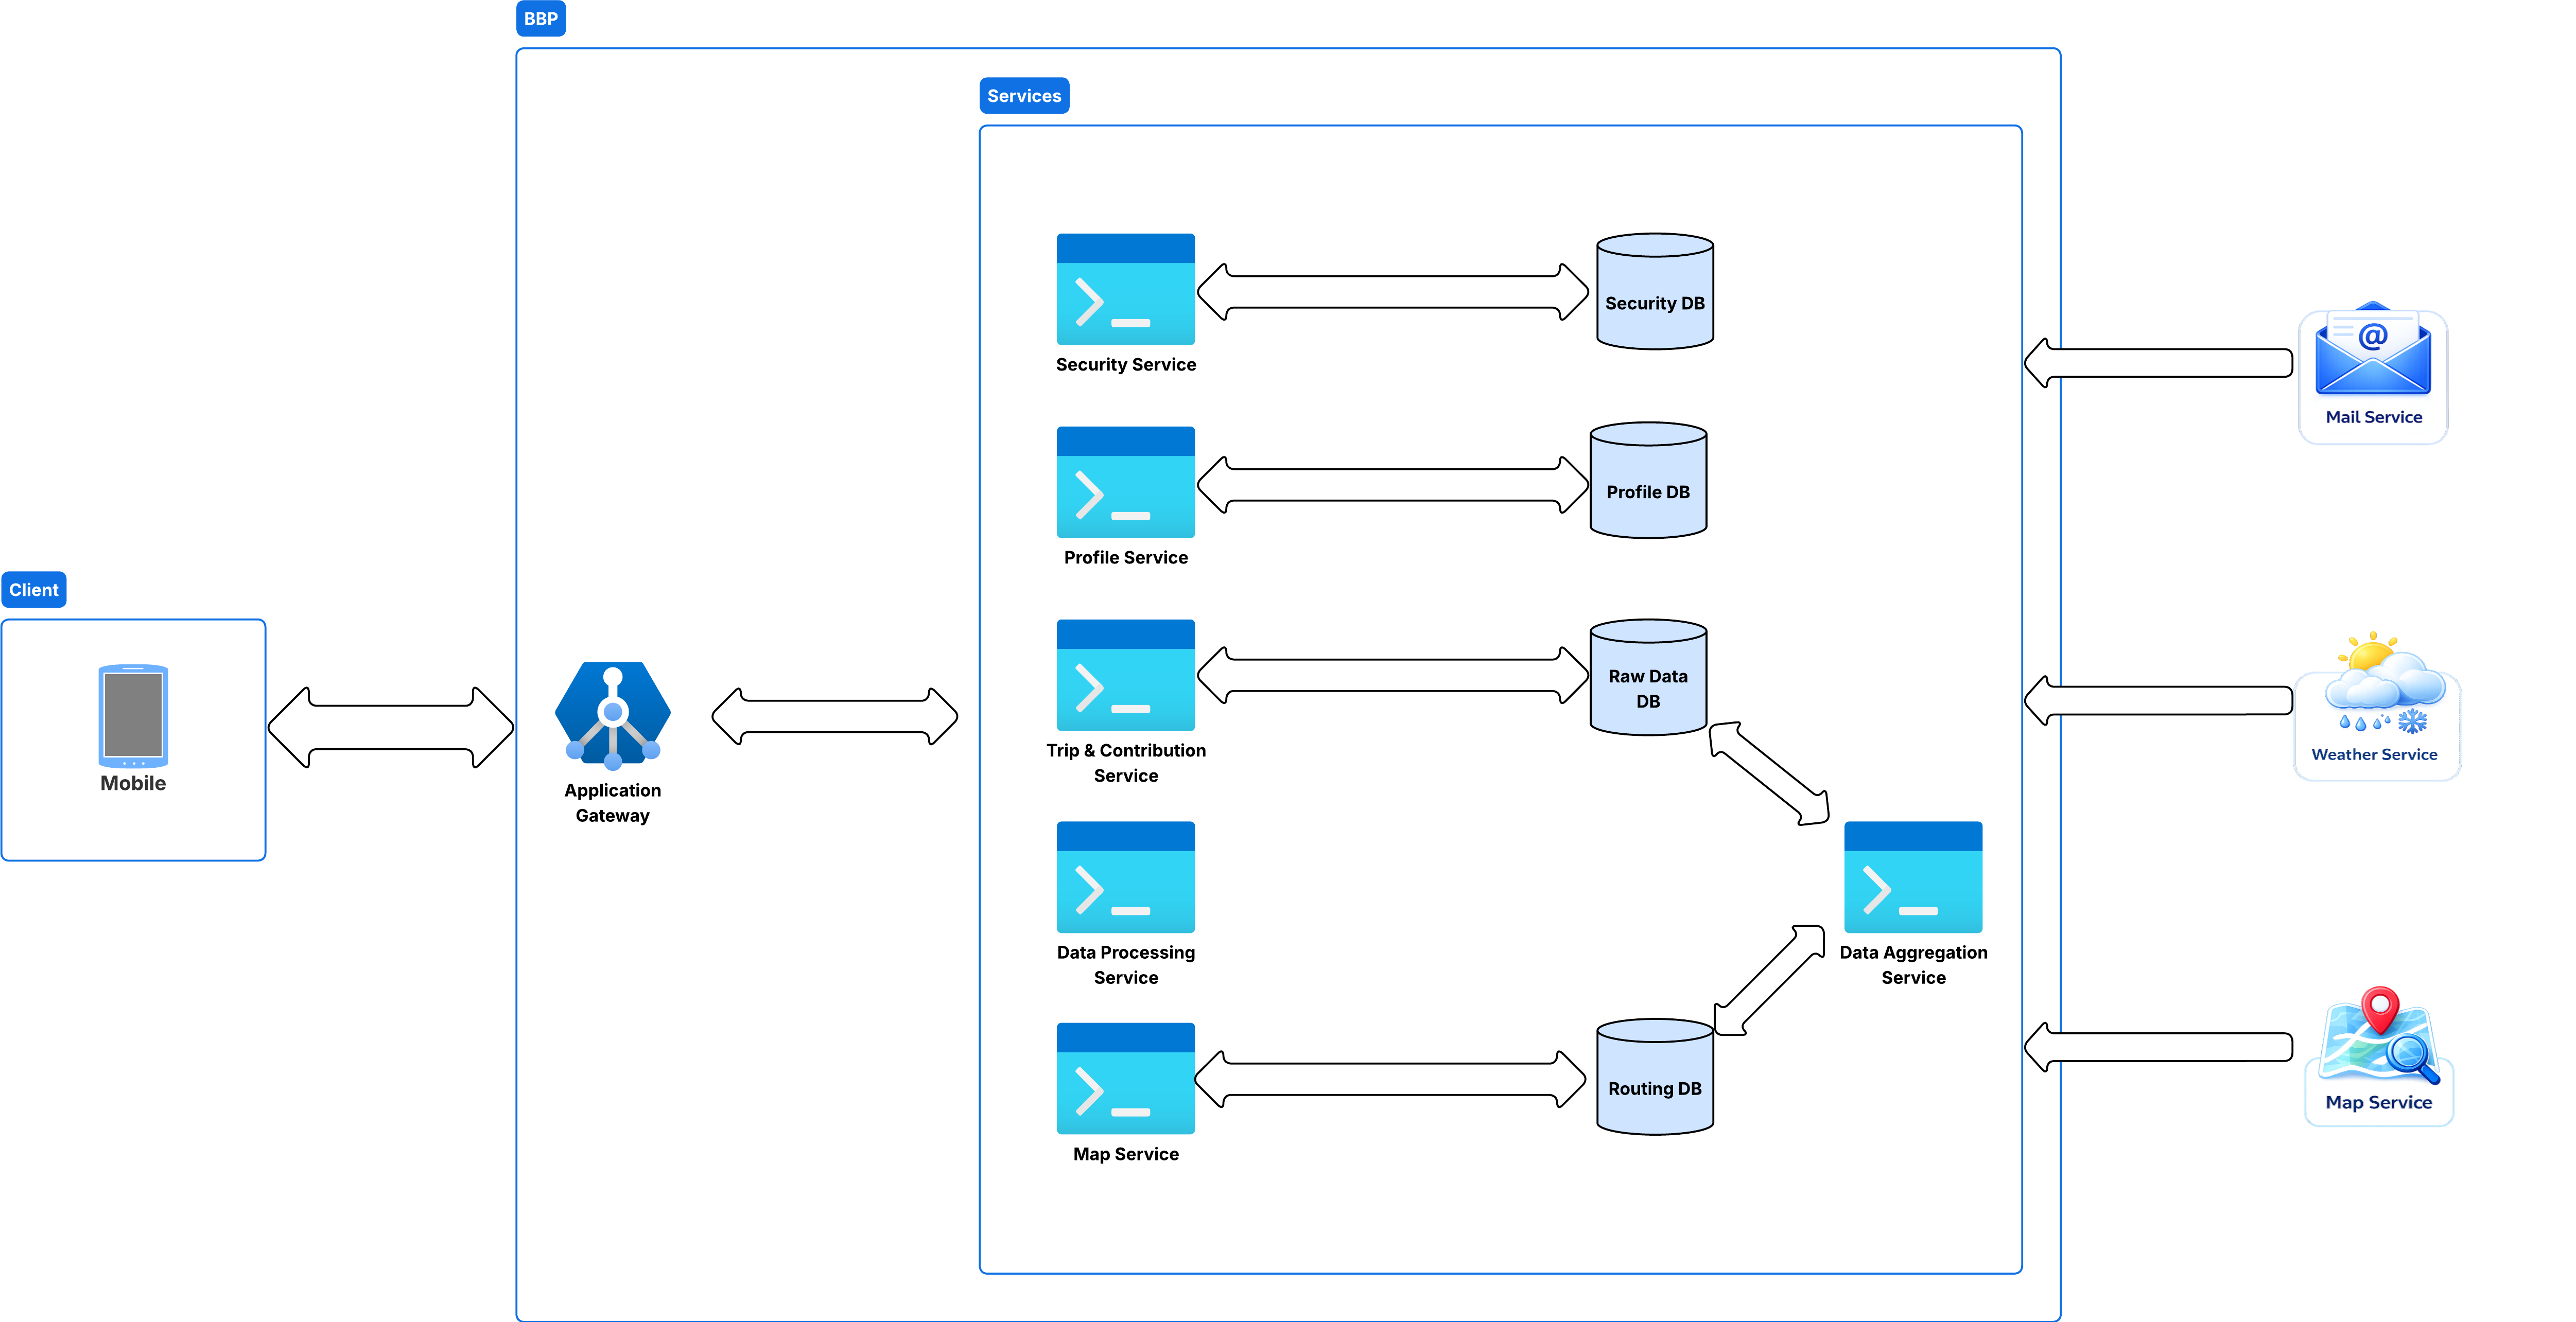
\includegraphics[width=1\linewidth]{DD/Images/Overview.png}
    \caption{High-level overview of the BBP system architecture.}
    \label{fig:overview}
\end{figure}



\label{subsec:components_description}


\section{Component View}
\label{sec: component_view}

In this section, the main components of the BBP system are presented, together with a concise description of their responsibilities. Each component is derived from the product functions introduced in Section 2.2 of the RASD.  
Components addressing closely related functionalities are grouped together into higher-level services, in order to improve modularity, separation of concerns, and maintainability of the system architecture.


\subsection{Component Diagram}
\label{subsec:component_diagram}
\begin{figure} [H]
    \begin{center}
        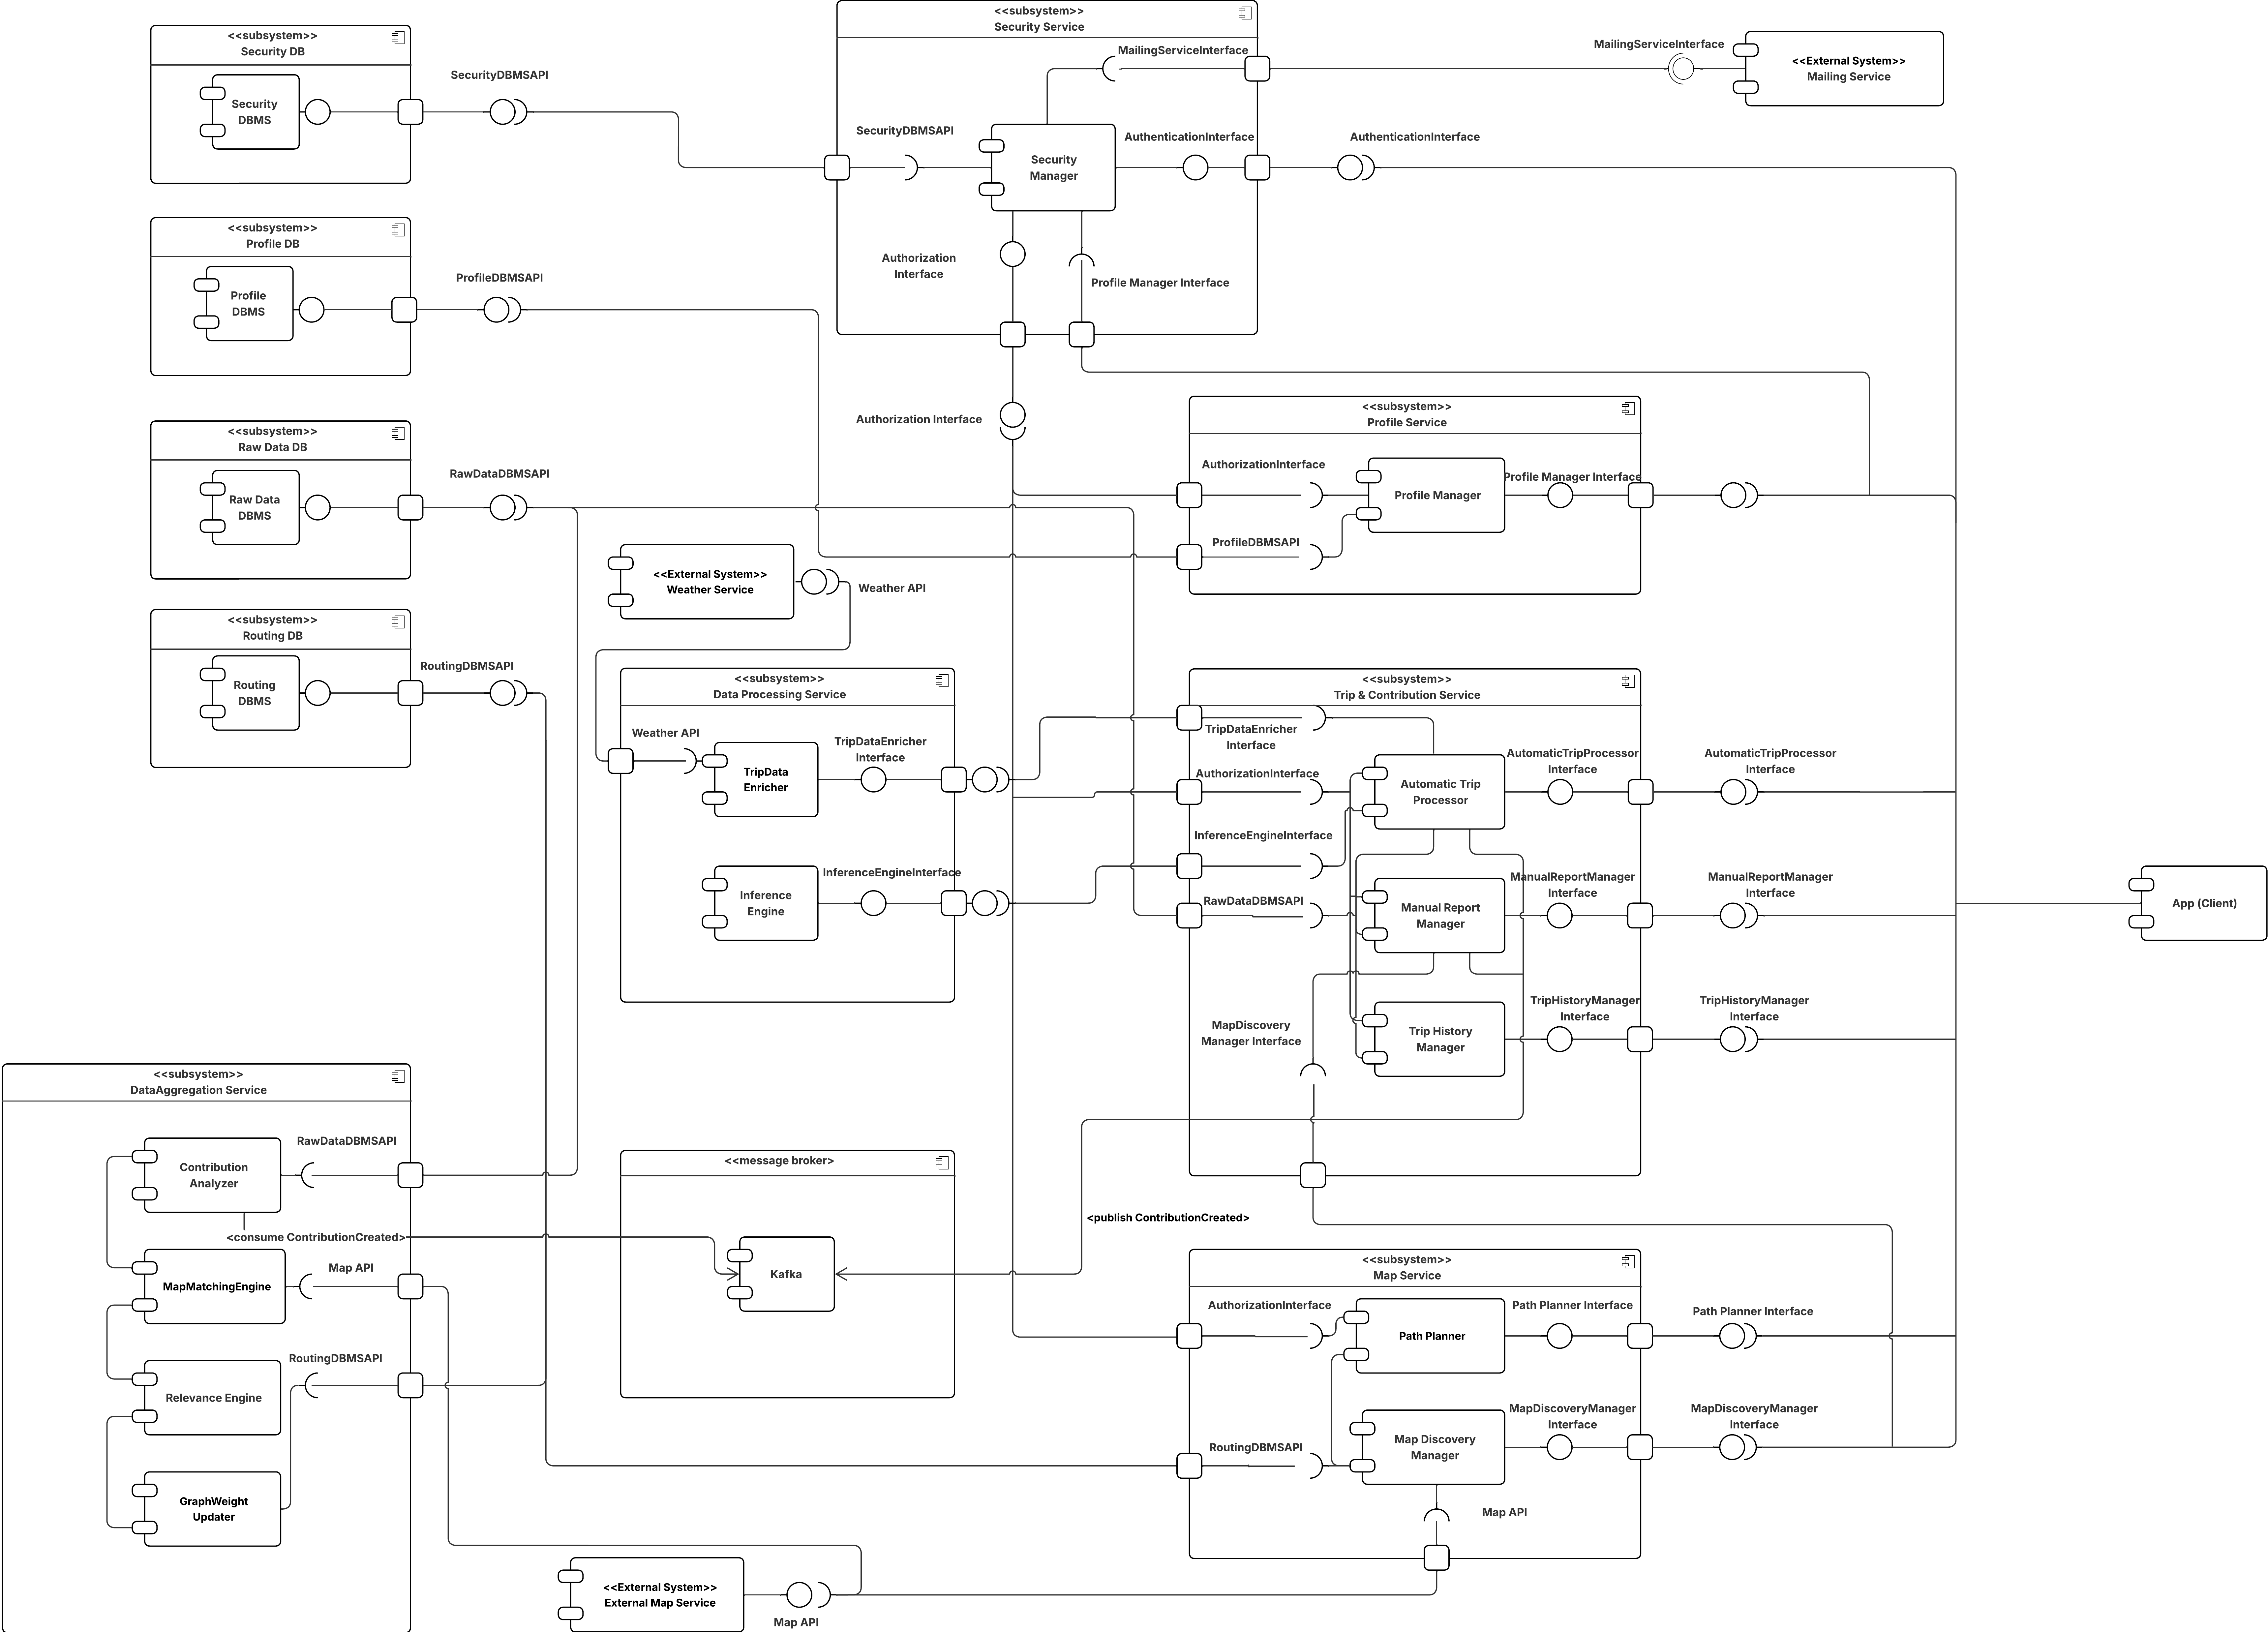
\includegraphics[width=0.95\linewidth]{DD/Images/component_diagram.png}
        \caption{Component diagram of the BBP system.}
        \label{fig:component_diagram}
    \end{center}
\end{figure}

\subsection{Components Description}
\label{subsec:components_description}

Each component is intended as a cohesive logical unit that encapsulates a set of collaborating internal elements to deliver the specified functionalities.
The internal structure and implementation details of these elements are deliberately left unspecified, as they are not binding with respect to the overall system architecture, provided that each component satisfies the defined responsibilities.
For the sake of clarity and readability, infrastructural elements such as the API Gateway are not represented explicitly in the component diagram, but are considered implicitly as part of the system’s communication infrastructure.

\begin{enumerate}

    \item \textbf{SecurityManager:}  
    This component is responsible for authentication and authorization of users accessing the system. It manages login operations and token validation, ensuring that only authenticated users can invoke protected functionalities. The SecurityManager interacts with the SecurityDBMS, a relational DBMS storing credentials and authentication-related information, and exposes authorization interfaces used by the other microservices.

    \item \textbf{MailingService:}  
    This component handles email-based communications required by the platform, such as account verification messages. It is invoked by the SecurityManager during registration procedures in order to decouple authentication logic from communication concerns.

    \item \textbf{ProfileManager:}  
    This component manages user profile information, including personal data and preferences that influence route ranking and visualization. It provides operations to retrieve and update profiles and persists such data through the ProfilesDBMS, a relational DBMS. All profile-related operations require prior authorization.

    \item \textbf{AutomaticTripProcessor:}  
    This component manages the lifecycle of automatically recorded trips. Trip recording is performed locally on the client, which collects GPS traces and sensor data until the user explicitly terminates the trip. When the user decides to save the recorded trip, the collected data is sent to the AutomaticTripProcessor, which invokes the Inference Engine to analyze sensor data and automatically generate preliminary contributions (e.g., road anomalies or quality indicators). The inferred data is then forwarded to the TripData Enricher, which computes advanced trip statistics and enriches the trip with contextual information such as weather conditions by interacting with an external Weather Service.
    
    The processed trip is returned to the AutomaticTripProcessor, which stores a draft copy in the RawDataDBMS, marked as non-definitive, and sends the enriched trip back to the client. At this stage, the user can review, modify, add, or remove contributions, including those generated automatically. Depending on user choice, the trip can be discarded, saved as private, or published. If the trip is published, the AutomaticTripProcessor stores the definitive copy marked as public and publishes a corresponding event to the Kafka message broker, enabling asynchronous aggregation and merging processes.
    
    It is worth noting that, at this stage, contributions are still associated with raw geographic coordinates. The association of each contribution to a specific street segment—considered the atomic working unit of the system—is performed later through a map matching process. This operation relies on external map data providers (e.g., OpenStreetMap) and is handled asynchronously by the Data Aggregation Service during the aggregation phase.


    \item \textbf{ManualReportManager:}  
    This component handles user-generated manual reports and manually declared trips. Users can submit individual reports or manually describe a completed trip through map interaction. During this process, the ManualReportManager interacts with the Map Discovery Manager, which leverages an external map service to determine the geographic coordinates corresponding to the user’s selection.
    
    Manual submissions do not undergo inference or data enrichment and are stored directly in the RawDataDBMS using raw geographic coordinates. Depending on user choice, the data can be saved as private or published. If published, the ManualReportManager generates an event that is sent to the Kafka message broker.
    
    Similarly to automatically generated contributions, the association of manual contributions to the system’s atomic working unit (street segments) is performed asynchronously by the backend through a unified map matching process. This design choice allows the map matching logic to be implemented only once and shared across both manual and automatic contributions, ensuring consistency and scalability.


    \item \textbf{TripHistoryManager:}  
    This component provides functionalities to retrieve, list, and delete previously recorded trips. It accesses the RawDataDBMS to manage persisted trip data according to user requests.

    \item \textbf{Inference Engine:}  
    This component analyzes raw sensor data associated with automatically recorded trips in order to infer meaningful information, such as anomalies, obstacles, or road quality indicators. 

    \item \textbf{TripData Enricher:}  
    This component enriches trip data with additional contextual and computed information. It integrates external data sources, such as weather conditions, by invoking an external Weather Service through REST calls. In addition, it computes advanced trip statistics (e.g., distance, duration, speed-related and performance metrics) based on the reconstructed path and collected raw data.  
    The TripData Enricher is modeled as a separate component to allow future extensions with additional enrichment sources without impacting other parts of the system.

    \item \textbf{ContributionAnalyzer:}  
    This component consumes publication events from the Kafka message broker corresponding to newly published trips and manual reports. Rather than processing each contribution immediately, the ContributionAnalyzer applies internal aggregation policies—such as time-based windows or contribution-count thresholds—to determine when a sufficient and meaningful set of data is available.
    
    Once the defined conditions are met, the component initiates the aggregation workflow by selecting the relevant contributions from the RawDataDBMS and coordinating subsequent processing steps, including map matching, relevance evaluation, and updates to the global routing representation. This design enables scalable, batch-oriented processing while preventing unnecessary or premature updates to the system’s global state.


    \item \textbf{MapMatchingEngine:}  
    This internal component of the Data Aggregation Service performs map matching operations by associating raw GPS traces and contribution coordinates to real-world street segments retrieved from the \textit{External Map Service}. Map matching is executed exclusively during the aggregation phase and is not persisted in the RawDataDBMS, as its sole purpose is to support the update of the global routing graph.

    \item \textbf{Relevance Engine:}  
    This component evaluates the relevance of individual contributions by considering factors such as consistency, frequency, and recency, determining which contributions should influence the system’s global state.

    \item \textbf{GraphWeight Updater:}  
    This component updates the weights and attributes of street segments stored in the RoutingDBMS, a graph-oriented DBMS. Updated weights reflect aggregated road conditions and bike-path suitability and are used to improve routing accuracy.

    \item \textbf{Path Planner:}  
    This component computes routes between two locations by executing routing algorithms over the graph stored in the RoutingDBMS. If no fully connected bike-path route exists, the Path Planner returns partial routes and coverage information, enabling graceful degradation.

    \item \textbf{Map Discovery Manager:}  
    This component provides map exploration functionalities. It retrieves base geographic map data from the\textit{External Map Service} and overlays the internal bike-path graph derived from user contributions, allowing users to visually inspect available bike paths within a given geographical area.

    \item \textbf{Kafka Message Broker:}  
    Kafka is used as an asynchronous messaging infrastructure to decouple trip publication and manual reporting from aggregation and merging processes. It enables background processing of published data without blocking user interactions and supports scalable, event-driven communication between microservices.

    \item \textbf{SecurityDBMS, ProfilesDBMS, RawDataDBMS, RoutingDBMS:}  
    The SecurityDBMS and ProfilesDBMS are relational databases used to store authentication credentials and user profile data, respectively. The RawDataDBMS is a document-oriented database that stores trips and contributions in flexible JSON-like structures. The RoutingDBMS is a graph database that stores street segments and their relationships, supporting efficient routing and graph-based analyses. All DBMS components are modeled as passive elements accessed directly by the corresponding microservices.

    \item \textbf{Weather Service (External System):}  
    This external system provides meteorological data used during the data enrichment process. It is accessed through standard REST calls and is not part of the core system architecture.

    \item \textbf{External Map Service (External System):}  
    This external system provides base geographic map data and road network information used by the BBP platform for visualization, coordinate resolution, and map matching operations. The system does not impose constraints on the specific map provider to be adopted; any compliant service exposing geographic and road network data through standard APIs can be integrated. OpenStreetMap is a suitable candidate due to its open nature and wide availability, but alternative providers may be employed without affecting the system architecture.

    \item \textbf{Mailing Service (External System):}  
    This external service is responsible for handling email-based communications required by the platform. It is used, for instance, to send account registration and verification emails containing time-limited confirmation links. The Mailing Service is invoked by the Security-related components and is decoupled from the core system logic, allowing different email delivery solutions to be adopted without impacting the overall architecture.


\end{enumerate}


\newpage


\section{Deployment View}

The system is deployed as a distributed service architecture to ensure high scalability, resilience, and modularity. Each layer is distributed across a collection of servers and has distinct responsibilities, as described below:
\begin{itemize}
    \item \textbf{Presentation Layer:} Represents the client in a traditional client–server architecture. Users interact with the BBP system through a mobile application, which is responsible for request initiation and data visualization.
    
    \item \textbf{Application Layer:} Hosts the services implementing the core business functionalities of the system. The deployment diagram illustrates a possible allocation of these services across different servers. The actual number of service instances and their distribution at runtime are dynamically determined by the orchestration platform, ensuring optimal resource utilization and resilience to varying traffic loads.
    
    \item \textbf{Service Management Layer:} Includes external and auxiliary services required by the BBP application. This layer comprises infrastructure services supporting the Data Layer, such as a replication and consistency service, as well as external services used to enrich application functionalities, such as map services or weather services providing route-related information.
    
    \item \textbf{Data Layer:} Handles persistent data storage using replicated database systems to guarantee fault tolerance and availability. The load balancer in the Service Management Layer ensures that requests are evenly distributed among database replicas.
\end{itemize}

Communication between layers occurs through REST APIs over HTTP/HTTPS, while interactions with the Data Layer rely on TCP/IP-based communication protocols.

\begin{figure} [H]
    \begin{center}
        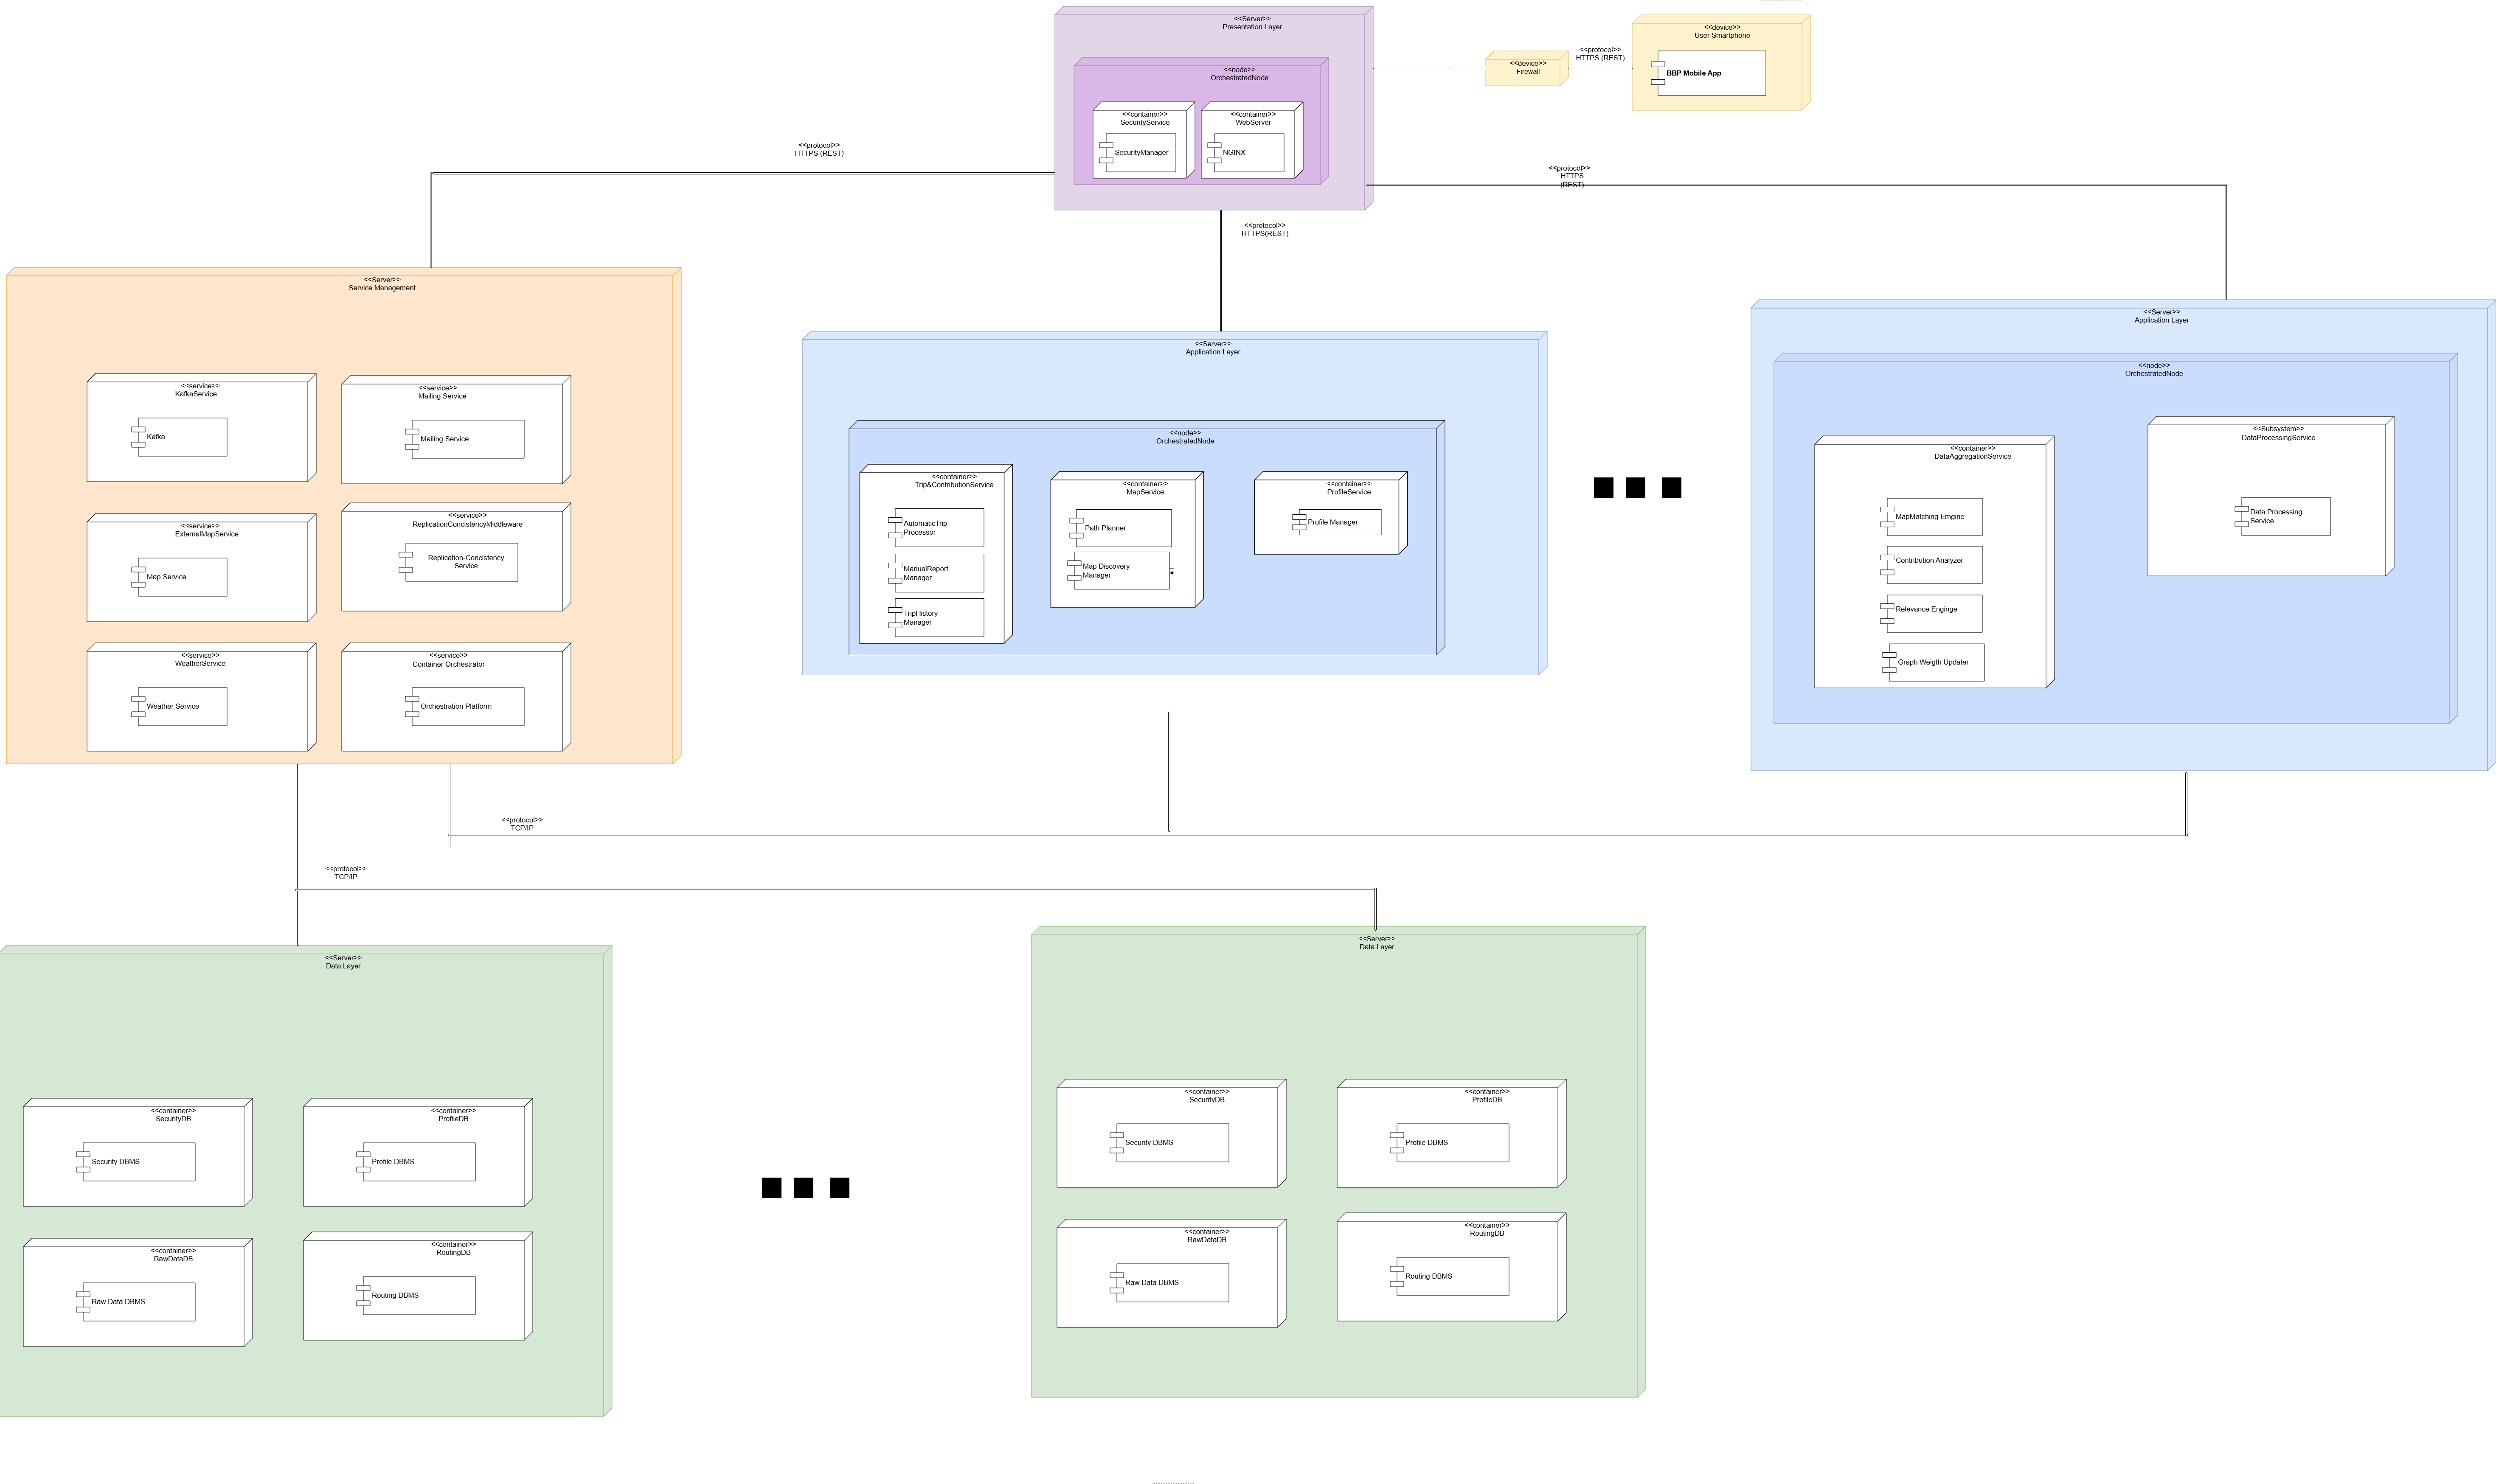
\includegraphics[width=0.95\linewidth]{DD/Images/Deployment_Diagram.png}
        \caption{UML Deployment Diagram}
        \label{fig:component_diagram}
    \end{center}
\end{figure}

\subsection{Detailed Layer Decisions}

The deployment architecture of the BBP system is designed to ensure high availability, scalability, and security through a containerized and distributed approach. The specific decisions regarding the layers are detailed below:

\begin{itemize}

    \item \textbf{Web Server and API Gateway:} 
    For clarity and performance, we selected \textbf{NGINX} as the web server acting as a reverse proxy and API Gateway. Deployed in a dedicated container, it serves as the single entry point for all client requests, hosting the API endpoints exposed to the mobile application. NGINX is responsible for forwarding requests to the appropriate microservices in the Application Layer. Additionally, it handles SSL/HTTPS termination, request filtering, and load balancing, distributing incoming traffic efficiently to prevent service overload and ensuring secure communication between the external world and the internal network. NGINX can be easily substituted by several separate dedicated components that each handle one of the functionalities.


    \item \textbf{Scalability and Containerization:} 
    The architecture follows a microservices inspired pattern where each main component runs in an isolated container. This isolation allows for independent horizontal scaling: the Orchestrator platform monitors resource consumption and incoming traffic patterns, dynamically adjusting the number of replicas for each service. For instance, during high-traffic events, the \textit{Trip Service} can be scaled up independently of the \textit{Profile Service}. In the Data Layer, replication is employed to improve read scalability, allowing the system to handle a high volume of concurrent read queries by distributing them across multiple database replicas.

    \item \textbf{Resiliency and Fault Tolerance:} 
    The container orchestration platform plays a crucial role in system reliability by managing failover mechanisms. If a service container crashes or becomes unresponsive, the orchestrator automatically detects the failure and restarts the instance or redirects traffic to healthy replicas. Furthermore, the decoupling of services via the \textbf{Kafka Message Broker} ensures that temporary unavailability of the \textit{Data Aggregation Service} does not block the ingestion of new trips, as events are queued and processed once the service is restored.

    \item \textbf{Orchestration Platform Considerations:} 
    While a specific technology is not strictly binding, a platform like \textbf{Kubernetes} is the reference choice for managing the container lifecycle. The orchestrator provides essential features such as server-side service discovery, allowing NGINX and internal services to locate each other dynamically without hard-coded IP addresses. It also manages internal networking and secret management, simplifying the operational overhead of maintaining a distributed infrastructure.

    \item \textbf{Polyglot Persistence and Data Consistency:} 
    The Data Layer is designed as a polyglot persistence environment, utilizing different DBMS technologies optimized for specific data types (Relational for profiles, Document for raw trips, Graph for routing). To ensure data availability, a Multi-Leader or Master-Slave replication strategy is adopted depending on the specific DBMS. This ensures that even in the event of a node failure, data remains accessible. Consistency is managed according to the data criticality: strict consistency is enforced for authentication and profiles (SecurityDBMS), while eventual consistency is accepted for the aggregation of crowd-sourced contributions into the routing graph.

\end{itemize}


\newpage

\section{Component Interfaces}
\label{sec:component_interfaces}

In this section the component interfaces defined for the system are described, highlighting for each one the expected inputs and outputs.

\subsection{REST API Endpoints}

Each microservice of the system exposes one or more interfaces, corresponding to the resource endpoints of the defined REST API. All protected endpoints require prior authorization through the \texttt{/authorization/validateToken} interface, which is implicitly invoked by the API Gateway before forwarding requests to the target microservice.

All API endpoints must be accessed through the HTTPS POST method, unless explicitly stated otherwise. Input parameters and output values are provided in JSON format within the request and response bodies.

To improve readability, only user-driven API calls are documented in this section.

The general structure of an API request is the following:

\texttt{https://DOMAIN/api/VERSION/INTERFACE/FUNCTION}

\subsubsection*{/authentication}

\begin{itemize}
    \item \texttt{/login} \\
    \textit{parameters:} \{ username: String, passwordHash: String \} \\
    \textit{responses:}
    \begin{itemize}
        \item \textbf{200 OK:} body: \{ accessToken: String, refreshToken: String \}
        \item \textbf{400 Bad Request:} body: \{ error: Enum(wrongCredentials) \}
    \end{itemize}

    \item \texttt{/refreshToken} \\
    \textit{parameters:} \{ refreshToken: String \} \\
    \textit{responses:}
    \begin{itemize}
        \item \textbf{200 OK:} body: \{ accessToken: String \}
    \end{itemize}

    \item \texttt{/logout} \\
    \textit{parameters:} \{ accessToken: String \} \\
    \textit{responses:}
    \begin{itemize}
        \item \textbf{204 No Content}
    \end{itemize}
\end{itemize}

\subsubsection*{/authorization}

\begin{itemize}
    \item \texttt{/validateToken} \\
    \textit{parameters:} \{ token: String \} \\
    \textit{responses:}
    \begin{itemize}
        \item \textbf{200 OK:} body: \{ authorized: true \}
        \item \textbf{401 Unauthorized:} body: \{ authorized: false \}
    \end{itemize}
\end{itemize}

\subsubsection*{/profiles}

\begin{itemize}
    \item \texttt{/getPreferences} \\
    \textit{parameters:} \{ userId: String \} \\
    \textit{responses:}
    \begin{itemize}
        \item \textbf{200 OK:} body: \{ preferences: MapPreferences \}
    \end{itemize}

    \item \texttt{/updatePreferences} \\
    \textit{parameters:} \{ preferences: MapPreferences \} \\
    \textit{responses:}
    \begin{itemize}
        \item \textbf{200 OK}
    \end{itemize}

    \item \texttt{/deleteAccount} \\
    \textit{parameters:} \{ userId: String, passwordHash: String \} \\
    \textit{responses:}
    \begin{itemize}
        \item \textbf{204 No Content}
        \item \textbf{400 Bad Request:} body: \{ error: Enum(wrongCredentials) \}
    \end{itemize}
\end{itemize}


\subsubsection*{/map}

\begin{itemize}
    \item \texttt{/getOverlay} \\
    \textit{parameters:} \{ boundingBox: BoundingBox, preferences: MapPreferences (optional) \} \\
    \textit{responses:}
    \begin{itemize}
        \item \textbf{200 OK:} body: \{ geoJson: GeoJSON \}
    \end{itemize}

    \item \texttt{/getSegments} \\
    \textit{parameters:} \{ boundingBox: BoundingBox \} \\
    \textit{responses:}
    \begin{itemize}
        \item \textbf{200 OK:} body: \{ segments: [ StreetSegment ] \}
    \end{itemize}

    \item \texttt{/getSegmentDetails} \\
    \textit{parameters:} \{ segmentId: String \} \\
    \textit{responses:}
    \begin{itemize}
        \item \textbf{200 OK:} body: \{ segment: StreetSegment, obstacles: [ Contribution ] \}
    \end{itemize}

    \item \texttt{/getObstacleDetails} \\
    \textit{parameters:} \{ contributionId: String \} \\
    \textit{responses:}
    \begin{itemize}
        \item \textbf{200 OK:} body: \{ contribution: Contribution \}
    \end{itemize}

    \item \texttt{/calculateRoute} \\
    \textit{parameters:} \{ start: Coordinate, end: Coordinate, preferences: MapPreferences (optional) \} \\
    \textit{responses:}
    \begin{itemize}
        \item \textbf{200 OK:} body: \{ route: Route \}
    \end{itemize}
\end{itemize}
\footnote{
Due to the incremental and contribution-driven nature of bike path data, the PathFinder component is designed to never fail. When a fully connected route cannot be computed, the system returns the best available partial route together with metadata describing the uncovered portion, ensuring graceful degradation and preserving usability.
}
\subsubsection*{/trips/automatic}

\begin{itemize}
    \item \texttt{/submit} \\
    \textit{parameters:} \{ tripData: RawTripData \} \\
    \textit{responses:}
    \begin{itemize}
        \item \textbf{200 OK:} body: \{ enrichedTrip: TripPreview \}
    \end{itemize}

    \item \texttt{/save} \\
    \textit{parameters:} \{ tripId: String, isPublic: Boolean \} \\
    \textit{responses:}
    \begin{itemize}
        \item \textbf{200 OK}
    \end{itemize}

    \item \texttt{/discard} \\
    \textit{parameters:} \{ tripId: String \} \\
    \textit{responses:}
    \begin{itemize}
        \item \textbf{204 No Content}
    \end{itemize}
\end{itemize}

\subsubsection*{/reports/manual}

\begin{itemize}
    \item \texttt{/submit} \\
    \textit{parameters:} \{ reportData: ManualReport, isTrip: Boolean, isPublic: Boolean \} \\
    \textit{responses:}
    \begin{itemize}
        \item \textbf{200 OK}
    \end{itemize}
\end{itemize}

\subsubsection*{/trips/history}

\begin{itemize}
    \item \texttt{/list} \\
    \textit{parameters:} \{ userId: String \} \\
    \textit{responses:}
    \begin{itemize}
        \item \textbf{200 OK:} body: \{ trips: [ TripSummary ] \}
    \end{itemize}

    \item \texttt{/getDetails} \\
    \textit{parameters:} \{ tripId: String \} \\
    \textit{responses:}
    \begin{itemize}
        \item \textbf{200 OK:} body: \{ trip: Trip \}
    \end{itemize}
\end{itemize}

\subsection{Other Interfaces}

\paragraph{Kafka}The Kafka message broker is used exclusively for asynchronous, event-driven communication between backend services and does not expose REST interfaces. Internal communication between components belonging to the same microservice is not exposed and therefore omitted.

\paragraph{External Geographic Data Provider}
The system relies on an external geographic data provider to obtain base map information and road network data used for visualization and map matching operations. The architecture does not impose constraints on the specific provider to be adopted, as long as it exposes suitable geographic and topological information through standard APIs.

For instance, if OpenStreetMap were used as the external provider, its Overpass API could be leveraged to query low-level map elements such as nodes, ways, and relations. Through such APIs—based on a C-like query language—it is possible to associate raw geographic coordinates with corresponding road segments, thereby supporting backend map matching operations. These interactions are entirely internal to the backend components and are not exposed as REST APIs.







\newpage
\section{Runtime View}
\label{sec:runtime_view}

In this section, the dynamic behavior of the system is described. For each Use Case identified in Section 3.1 \textit{Use Cases and Activity Diagrams} of the RASD, the corresponding Sequence Diagram is provided, highlighting the interactions and messages exchanged between the involved components.

As in previous sections, irrelevant details are omitted for clarity. In particular, most client-side interactions between the User and the Client App (e.g., form filling or minor UI interactions), implicit authorization checks performed by the API Gateway, and extremely frequent operations such as calls to the \texttt{/authorization/validateToken} endpoint are not explicitly shown, as they would unnecessarily increase the complexity of the diagrams.

\newcounter{uc}
\setcounter{uc}{1}
\newcommand{\cuc}{\theuc\stepcounter{uc}}

\subsubsection*{SD\cuc. Sign Up}
\label{subsubsec:signup_sd}

The User initiates the sign-up process by clicking the ``Sign Up'' button on the homepage of the Client App and submitting the required registration data through the \texttt{/api/v1/authentication/login} interface. The request is forwarded by the API Gateway to the \texttt{SecurityManager}, which validates the completeness and correctness of the submitted information, including password security requirements.

The \texttt{SecurityManager} then queries the \texttt{SecurityDBMS} to verify whether the provided email address is already associated with an existing account. If the email is already registered, the sign-up process is interrupted and the User is redirected to the login page. If the validation is successful, the \texttt{SecurityManager} creates a new, unverified user account in the \texttt{SecurityDBMS} and invokes the \texttt{MailingService} to send a verification email containing a confirmation link with a limited validity period of 24 hours.

When the User receives the verification email and clicks on the confirmation link before its expiration, a request is issued to the \texttt{/api/v1/authentication/verifyProfile} endpoint. The \texttt{SecurityManager} marks the account as verified in the \texttt{SecurityDBMS} and grants the User access to the profile completion page. At this point, the User can insert the remaining personal information required to complete the profile, after which the account becomes fully active and the User is allowed to access the platform functionalities.

If the verification link expires before being used, the \texttt{SecurityManager} invalidates the link and removes the previously stored unverified account data from the \texttt{SecurityDBMS}, forcing the User to repeat the registration process.

\newpage

\begin{figure}[H]
    \centering
    % Cambia 0.7 con la dimensione che preferisci (es. 0.5, 0.8, ecc.)
    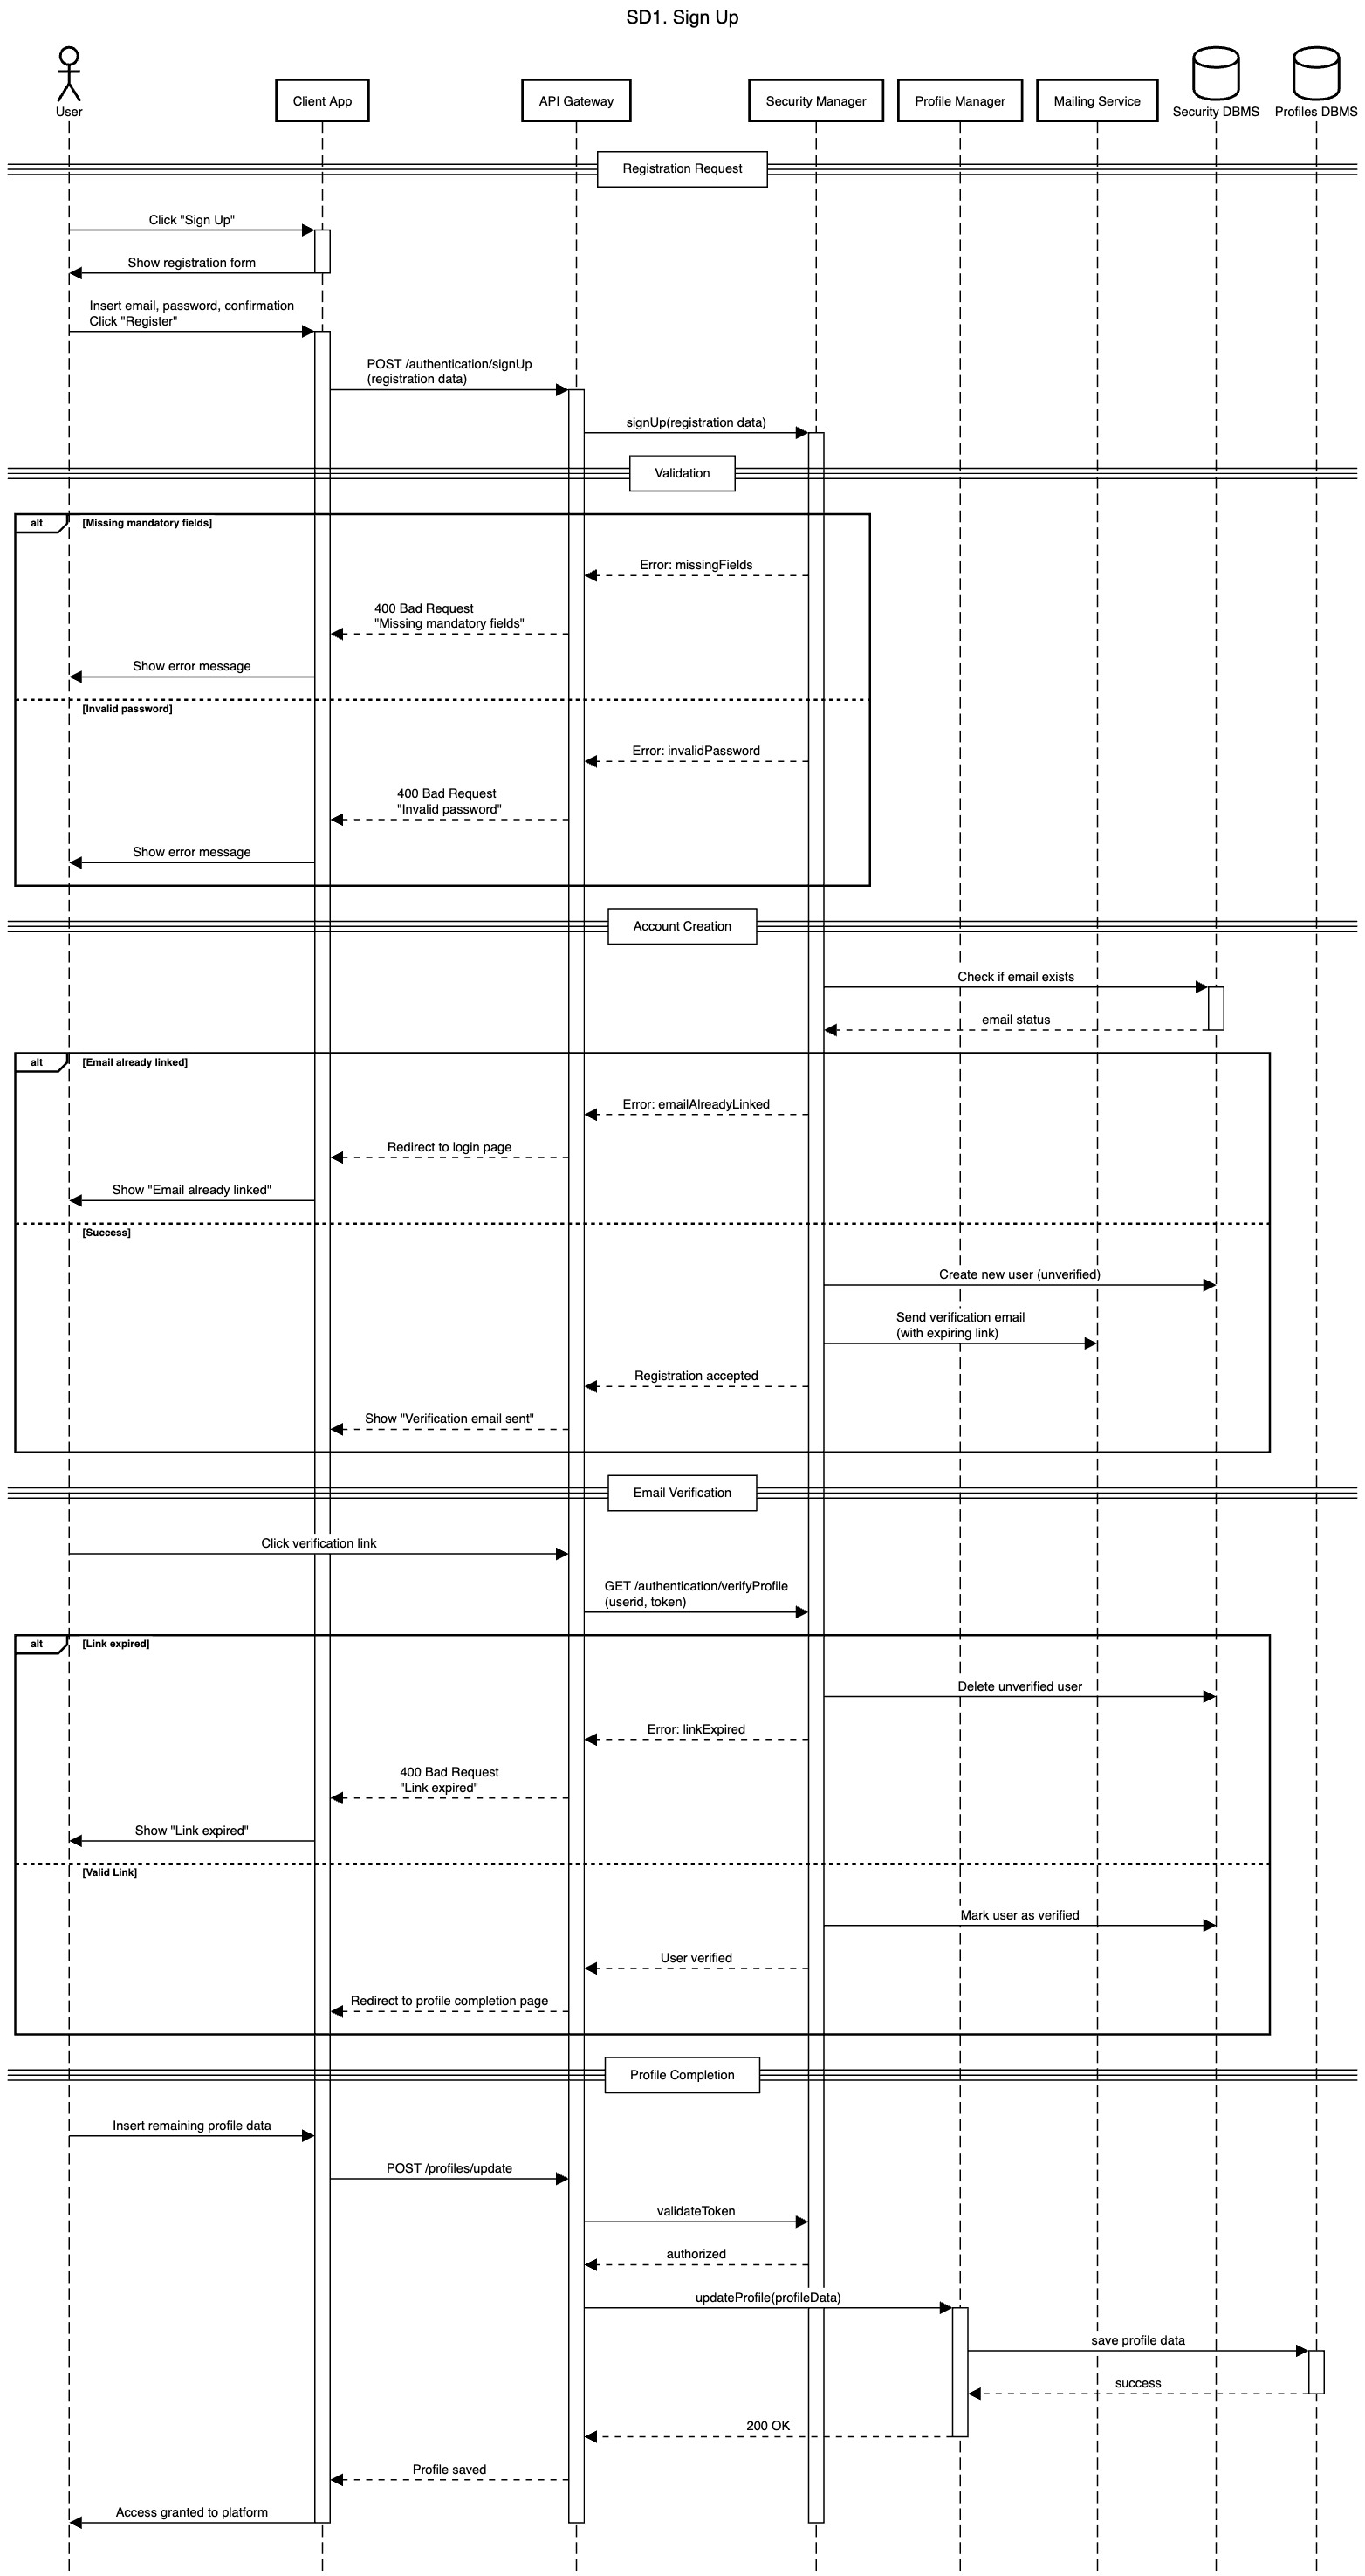
\includegraphics[width=0.75\linewidth]{DD/Images/sd/sd_signup.png}
    \caption{Sign Up}
    \label{fig:signup_sd}
\end{figure}

\newpage

\subsubsection*{SD\cuc. Sign In}
\label{subsubsec:signin_sd}

The User initiates the sign-in process by clicking the ``Sign In'' button on the homepage of the Client App and submitting their credentials through the \texttt{/api/v1/authentication/login} API endpoint. The request is routed by the API Gateway to the \texttt{SecurityManager}, which validates the provided credentials by querying the \texttt{SecurityDBMS}.

If the submitted credentials are not valid, the authentication process is immediately interrupted and the User is notified that the entered credentials are incorrect. Similarly, if the account associated with the provided email address has not yet been verified, the \texttt{SecurityManager} denies access and informs the User that the account is not verified.

If the credentials are valid and the account is verified, the \texttt{SecurityManager} completes the authentication process by generating the access tokens and checking whether the User profile is complete. If the profile is complete, the User is redirected to the Home page of the platform. Otherwise, the User is redirected to the profile completion page, where the missing personal information can be provided.

\newpage

\begin{figure}[H]
    \begin{center}
         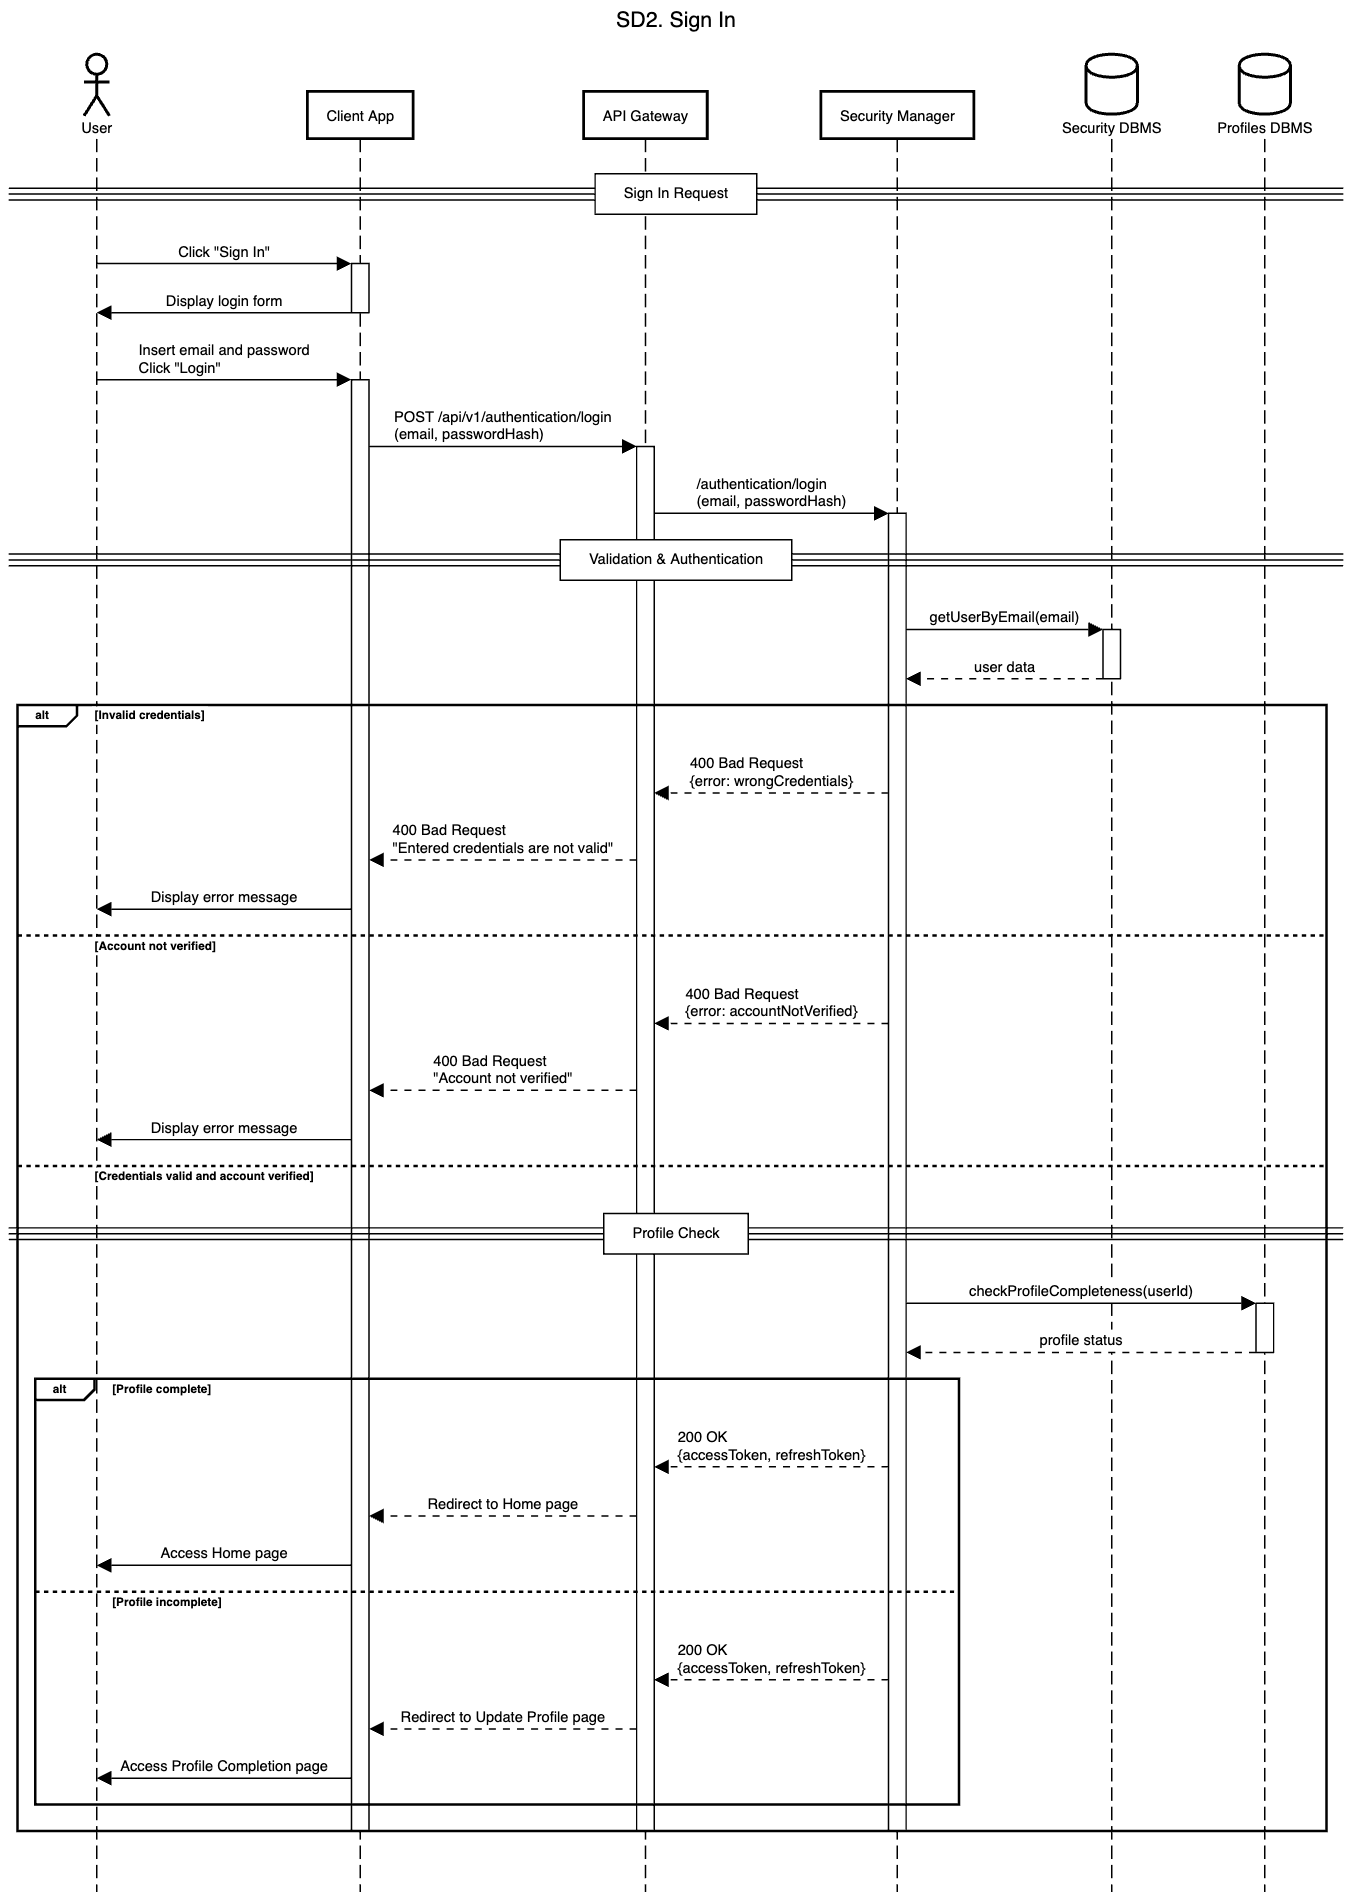
\includegraphics[width=1\linewidth]{DD/Images/sd/sd_signin.png}
         \caption{Sign In}
         \label{fig:signin_sd}
     \end{center}
\end{figure}

\newpage


\subsubsection*{SD\cuc. Delete Account}
\label{subsubsec:delete_account_sd}

The Registered User initiates the account deletion process by accessing the account settings page of the Client App and selecting the ``Delete account'' option. The system displays a warning explaining the consequences of account deletion and asks the User to confirm the operation. If the User cancels the process, no further action is performed and the User is returned to the account settings page.

If the User confirms the deletion, the system requires re-authentication by requesting the User’s credentials. The credentials are submitted through the \texttt{/api/v1/profiles/deleteAccount} API endpoint and forwarded by the API Gateway to the \texttt{SecurityManager}. The \texttt{SecurityManager} validates the provided credentials by querying the \texttt{SecurityDBMS}. If the credentials are not valid, the deletion process is aborted and the User is notified accordingly.

If the credentials are valid, the \texttt{SecurityManager} orchestrates the account deletion process. The User profile and preferences are removed from the \texttt{ProfilesDBMS}, all trips associated with the User are deleted from the \texttt{RawDataDBMS}, and authentication credentials are removed from the \texttt{SecurityDBMS}. Additionally, all active sessions and authentication tokens associated with the User are invalidated to prevent further access.

Published contributions are not removed during this process, as they have already been aggregated and merged into the routing graph and can no longer be uniquely associated with a specific User.

Finally, the system confirms the successful deletion of the account to the User, who is no longer able to access the platform using the previous credentials.

\newpage

\begin{figure}[H]
    \begin{center}
         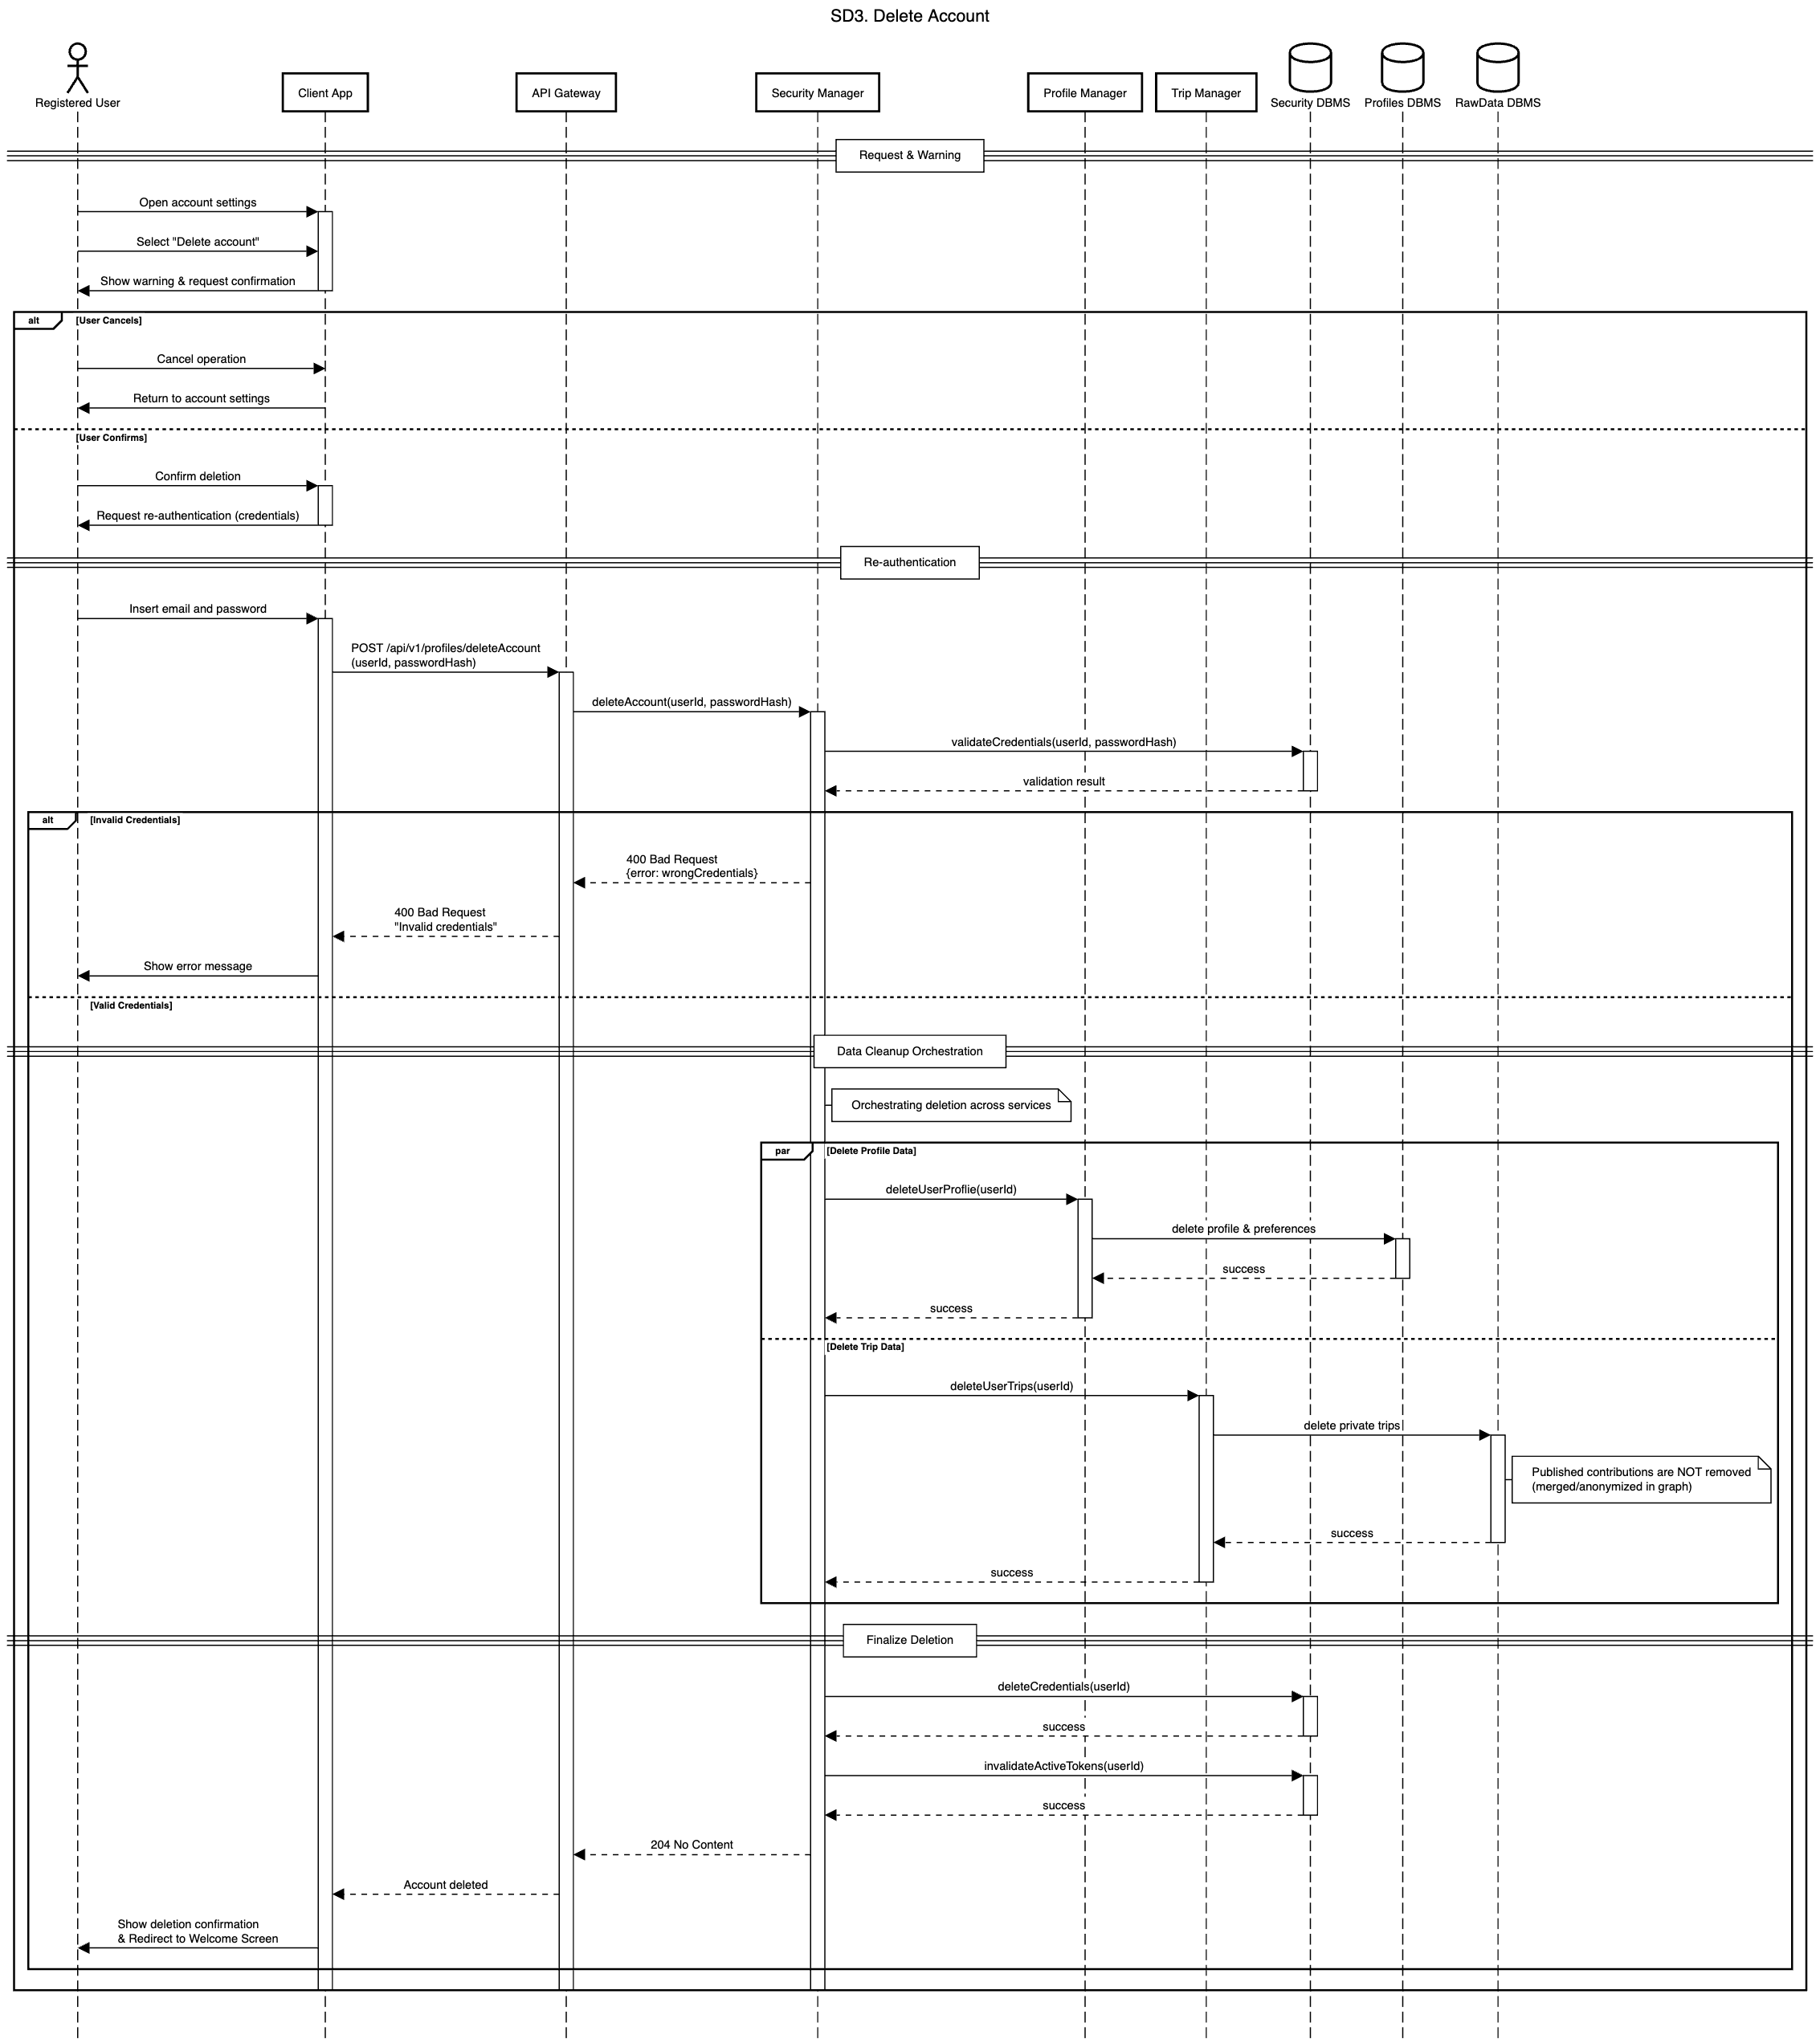
\includegraphics[width=1\linewidth]{DD/Images/sd/sd_delacc.png}
         \caption{Delete Account}
         \label{fig:delete_account_sd}
     \end{center}
\end{figure}

\newpage

\subsubsection*{SD\cuc. Logout}
\label{subsubsec:logout_sd}

The User initiates the logout process by clicking the ``Logout'' button within the Client App. The logout request is sent through the \texttt{/api/v1/authentication/logout} API endpoint and forwarded by the API Gateway to the \texttt{SecurityManager}.

Upon receiving the request, the \texttt{SecurityManager} invalidates the authentication token associated with the User by updating the \texttt{SecurityDBMS}, effectively terminating the active session. Once the token has been invalidated, the system confirms the successful logout operation.

Finally, the User is redirected to the Home screen of the platform and is no longer authenticated, preventing access to protected functionalities until a new login is performed.

\newpage

\begin{figure}[H]
    \begin{center}
         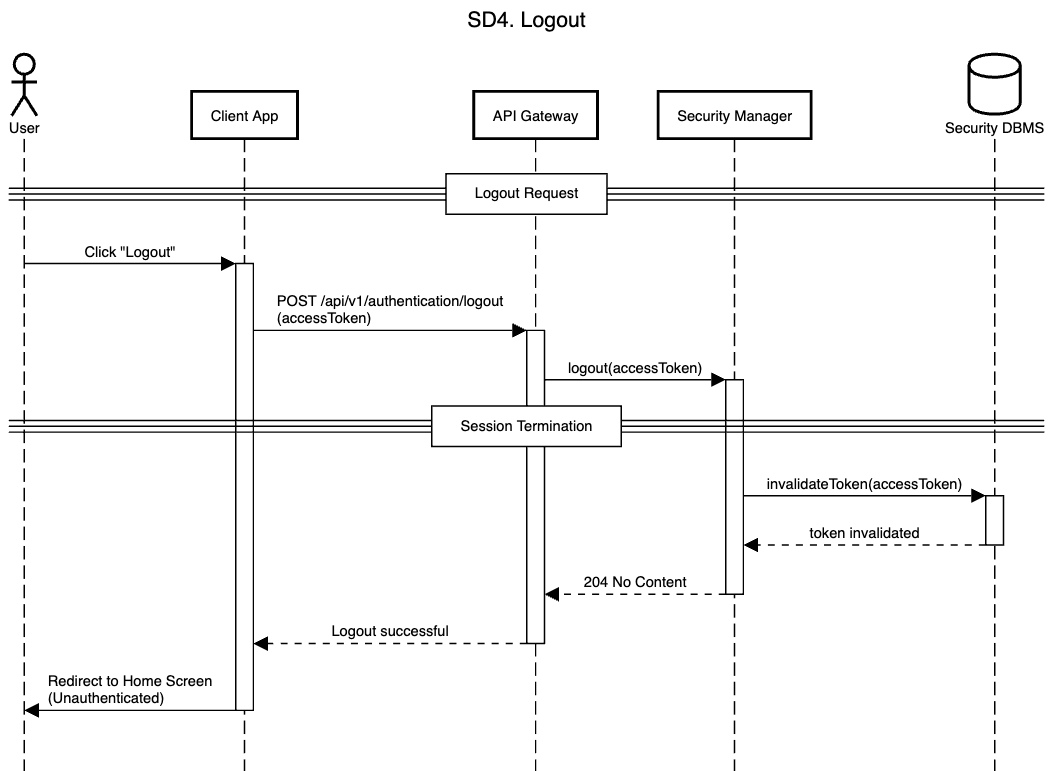
\includegraphics[width=1\linewidth]{DD/Images/sd/sd_logout.png}
         \caption{Logout}
         \label{fig:logout_sd}
     \end{center}
\end{figure}

\newpage

\subsubsection*{SD\cuc. Edit Profile}
\label{subsubsec:edit_profile_sd}

The Registered User accesses the profile management section of the Client App by clicking on the ``Profile'' area and selecting the ``Edit profile'' option. The system retrieves the current profile information and visualization preferences by invoking the \texttt{/api/v1/profiles/getPreferences} API endpoint, which is forwarded by the API Gateway to the \texttt{ProfileManager}. The retrieved data is then displayed to the User in an editable form.

The User updates the desired personal information and preferences, such as path visualization filters derived from previous trips, and confirms the changes by clicking the ``Apply'' button. The updated data is submitted through the \texttt{/api/v1/profiles/updatePreferences} API endpoint and handled by the \texttt{ProfileManager}.

The \texttt{ProfileManager} validates the submitted changes, checking both data consistency and supported preference values. If the validation fails, the update process is aborted and the User is notified that the provided information is not valid. No modification is applied to the stored data.

If the submitted data is valid, the \texttt{ProfileManager} updates the User profile and preferences in the \texttt{ProfilesDBMS}. Upon successful completion of the operation, the system notifies the User that the profile has been successfully updated, ensuring that the stored information remains consistent across the platform.

\newpage

\begin{figure}[H]
    \begin{center}
         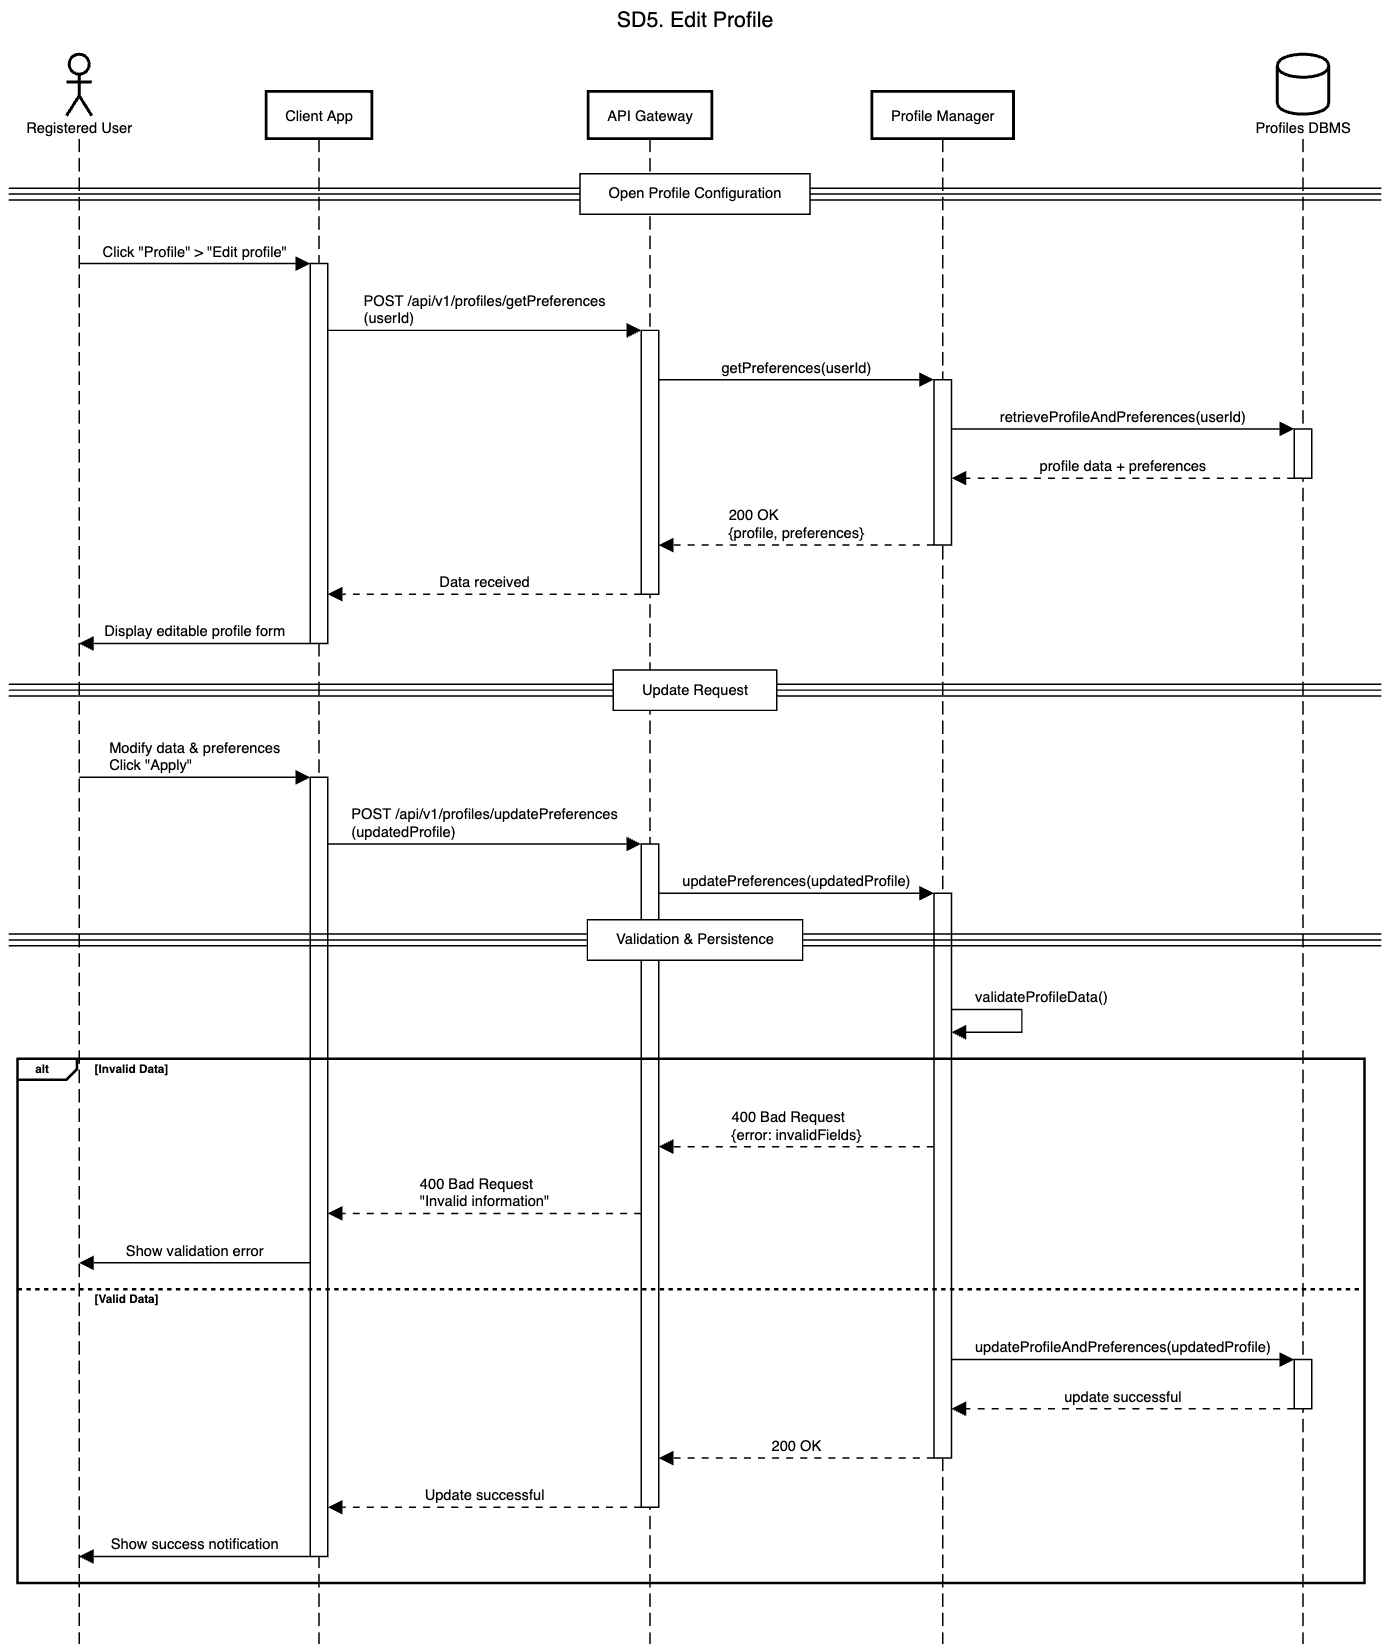
\includegraphics[width=1\linewidth]{DD/Images/sd/sd_editprofile.png}
         \caption{Edit Profile}
         \label{fig:edit_profile_sd}
     \end{center}
\end{figure}

\newpage

\subsubsection*{SD\cuc. View Trip History}
\label{subsubsec:view_trip_history_sd}

The Registered User accesses the trip history section of the Client App by selecting the ``My trips'' option. The system retrieves the list of trips associated with the User by invoking the \texttt{/api/v1/trips/history/list} API endpoint, which is forwarded by the API Gateway to the \texttt{TripHistoryManager}. The \texttt{TripHistoryManager} queries the \texttt{RawDataDBMS} to retrieve all stored trips belonging to the User.

If no trips are available, the system displays an empty list together with an informative message. Otherwise, the list of available trips is shown to the User, who can select one of them to inspect its details.

When a trip is selected, the Client App invokes the \texttt{/api/v1/trips/history/getDetails} API endpoint to retrieve the full trip data, including its associated contributions. The retrieved information is displayed to the User.

If the selected trip has no associated contributions, the system simply shows the trip data without triggering any further action. If contributions are present, the User may choose to publish them. In this case, the system iteratively processes each contribution, publishing them one at a time. Each publication generates an asynchronous event that is forwarded to the Kafka message broker, allowing the Data Aggregation Service to incrementally merge the contribution data and update the routing graph according to the defined merging and update policies as detailed in the following sequence diagram \textit{Publish Contribution}.

Once all selected contributions have been processed, control is returned to the trip view, allowing the User to continue browsing the application.

\newpage

\begin{figure}[H]
    \centering
    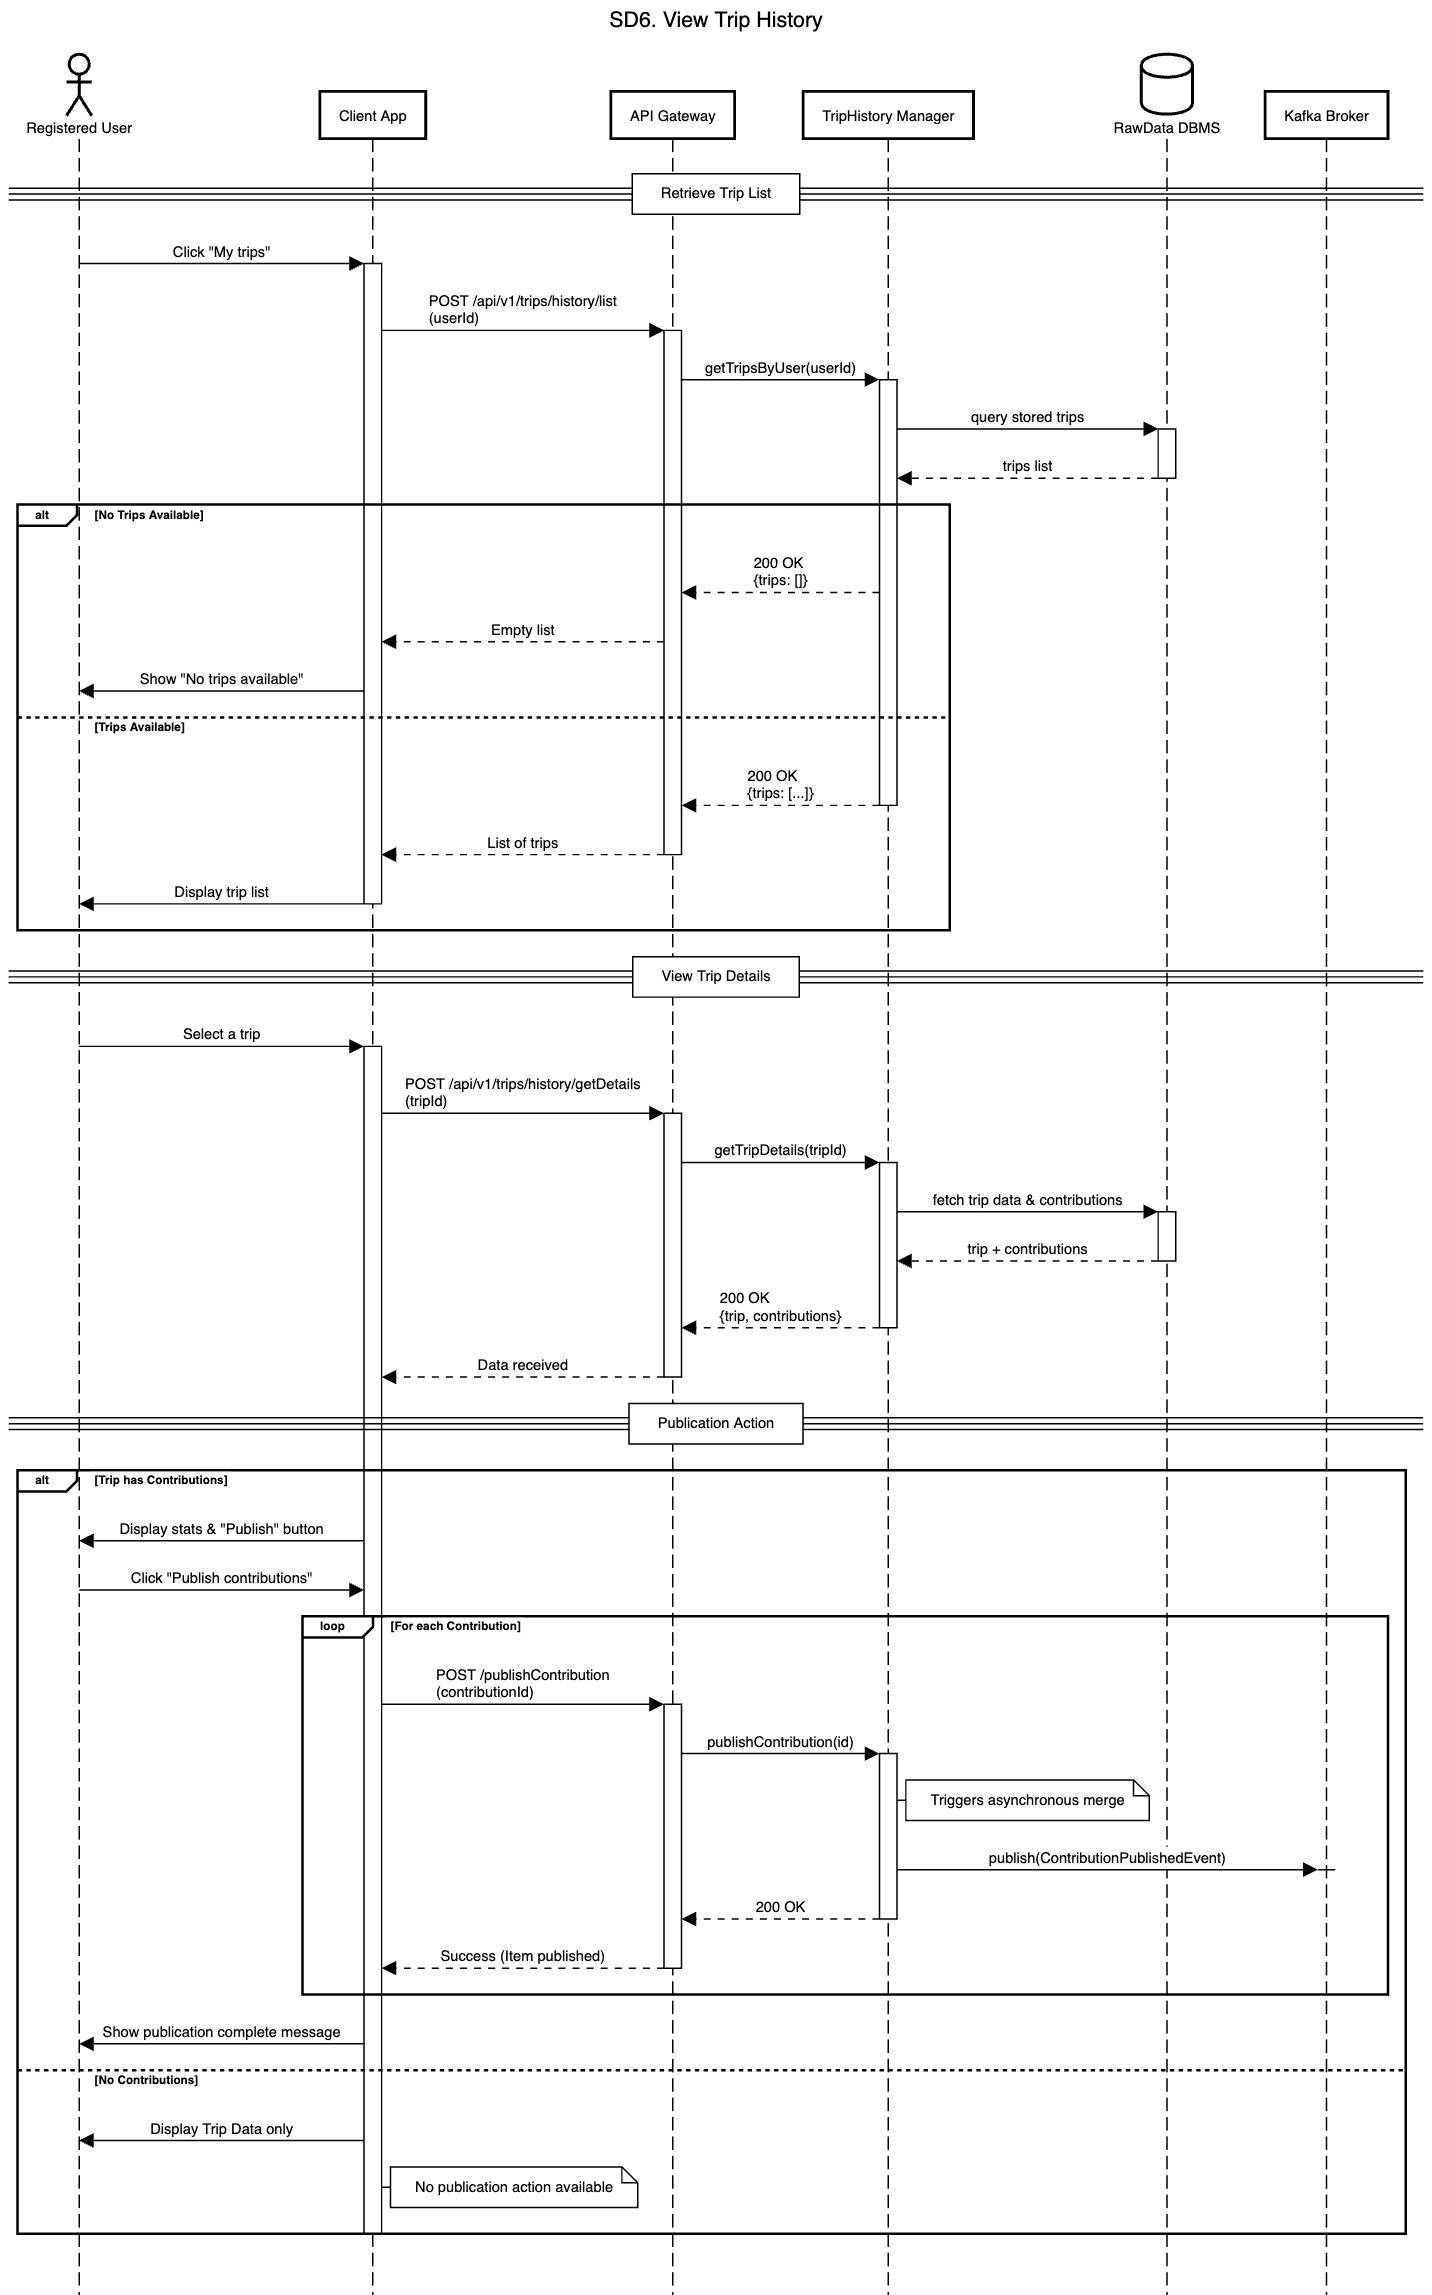
\includegraphics[width=0.85\linewidth]{DD/Images/sd/sd_viewhistory.png}
    \caption{View Trip History}
    \label{fig:view_trip_history_sd}
\end{figure}

\newpage


\subsubsection*{SD\cuc. Publish Contribution}
\label{subsubsec:publish_contribution_sd}

This use case describes the asynchronous processing and merging of a Contribution into the routing graph. It is not directly initiated by the User, but is triggered by other use cases (e.g., viewing the trip history or publishing an automatic or manual trip) when a Contribution is marked as public. Upon publication, the producing service emits a \texttt{ContributionPublishedEvent} to the Kafka message broker.

The ContributionAnalyzer periodically consumes events from Kafka and retrieves the corresponding Contribution data from the \texttt{RawDataDBMS}. The ContributionAnalyzer component first validates the Contribution, ensuring that all mandatory data is present and that the spatial and temporal information is consistent. If the Contribution is not valid, the process is aborted and the merge status of the Contribution is marked as \texttt{FAILED}, without modifying any existing path information.

If the Contribution is valid, the  \texttt{ContributionAnalyzer} sends a request to the  \texttt{MapMatchingEngine} which retrieves a list of Street segments form external map services, associates the contribution to the correct segment returning it to the  \texttt{ContributionAnalyzer} who retrieves all existing Contributions referring to the same street or path segment from the \texttt{RawDataDBMS}. The  \texttt{RelevanceEngine} then filters the retrieved data, discarding outliers and selecting only the most relevant Contributions according to predefined criteria such as severity, frequency, and recency.

The  \texttt{GraphWeightUpdater} applies a weighted incremental aggregation policy to merge the new Contribution with the existing information and updates the corresponding segment weight in the \texttt{RoutingDBMS}. This approach allows the routing graph to be updated incrementally and efficiently, without reprocessing the entire dataset.

Finally, upon successful completion of the merge process, the Contribution is marked as \texttt{MERGED} in the \texttt{RawDataDBMS}. Publishing a Contribution and merging it into the routing graph are treated as two distinct concerns: publication is the result of an explicit User action, while merging is handled asynchronously by the system to ensure scalability, responsiveness, and eventual consistency of the routing data.

\newpage

\begin{figure}[H]
    \begin{center}
         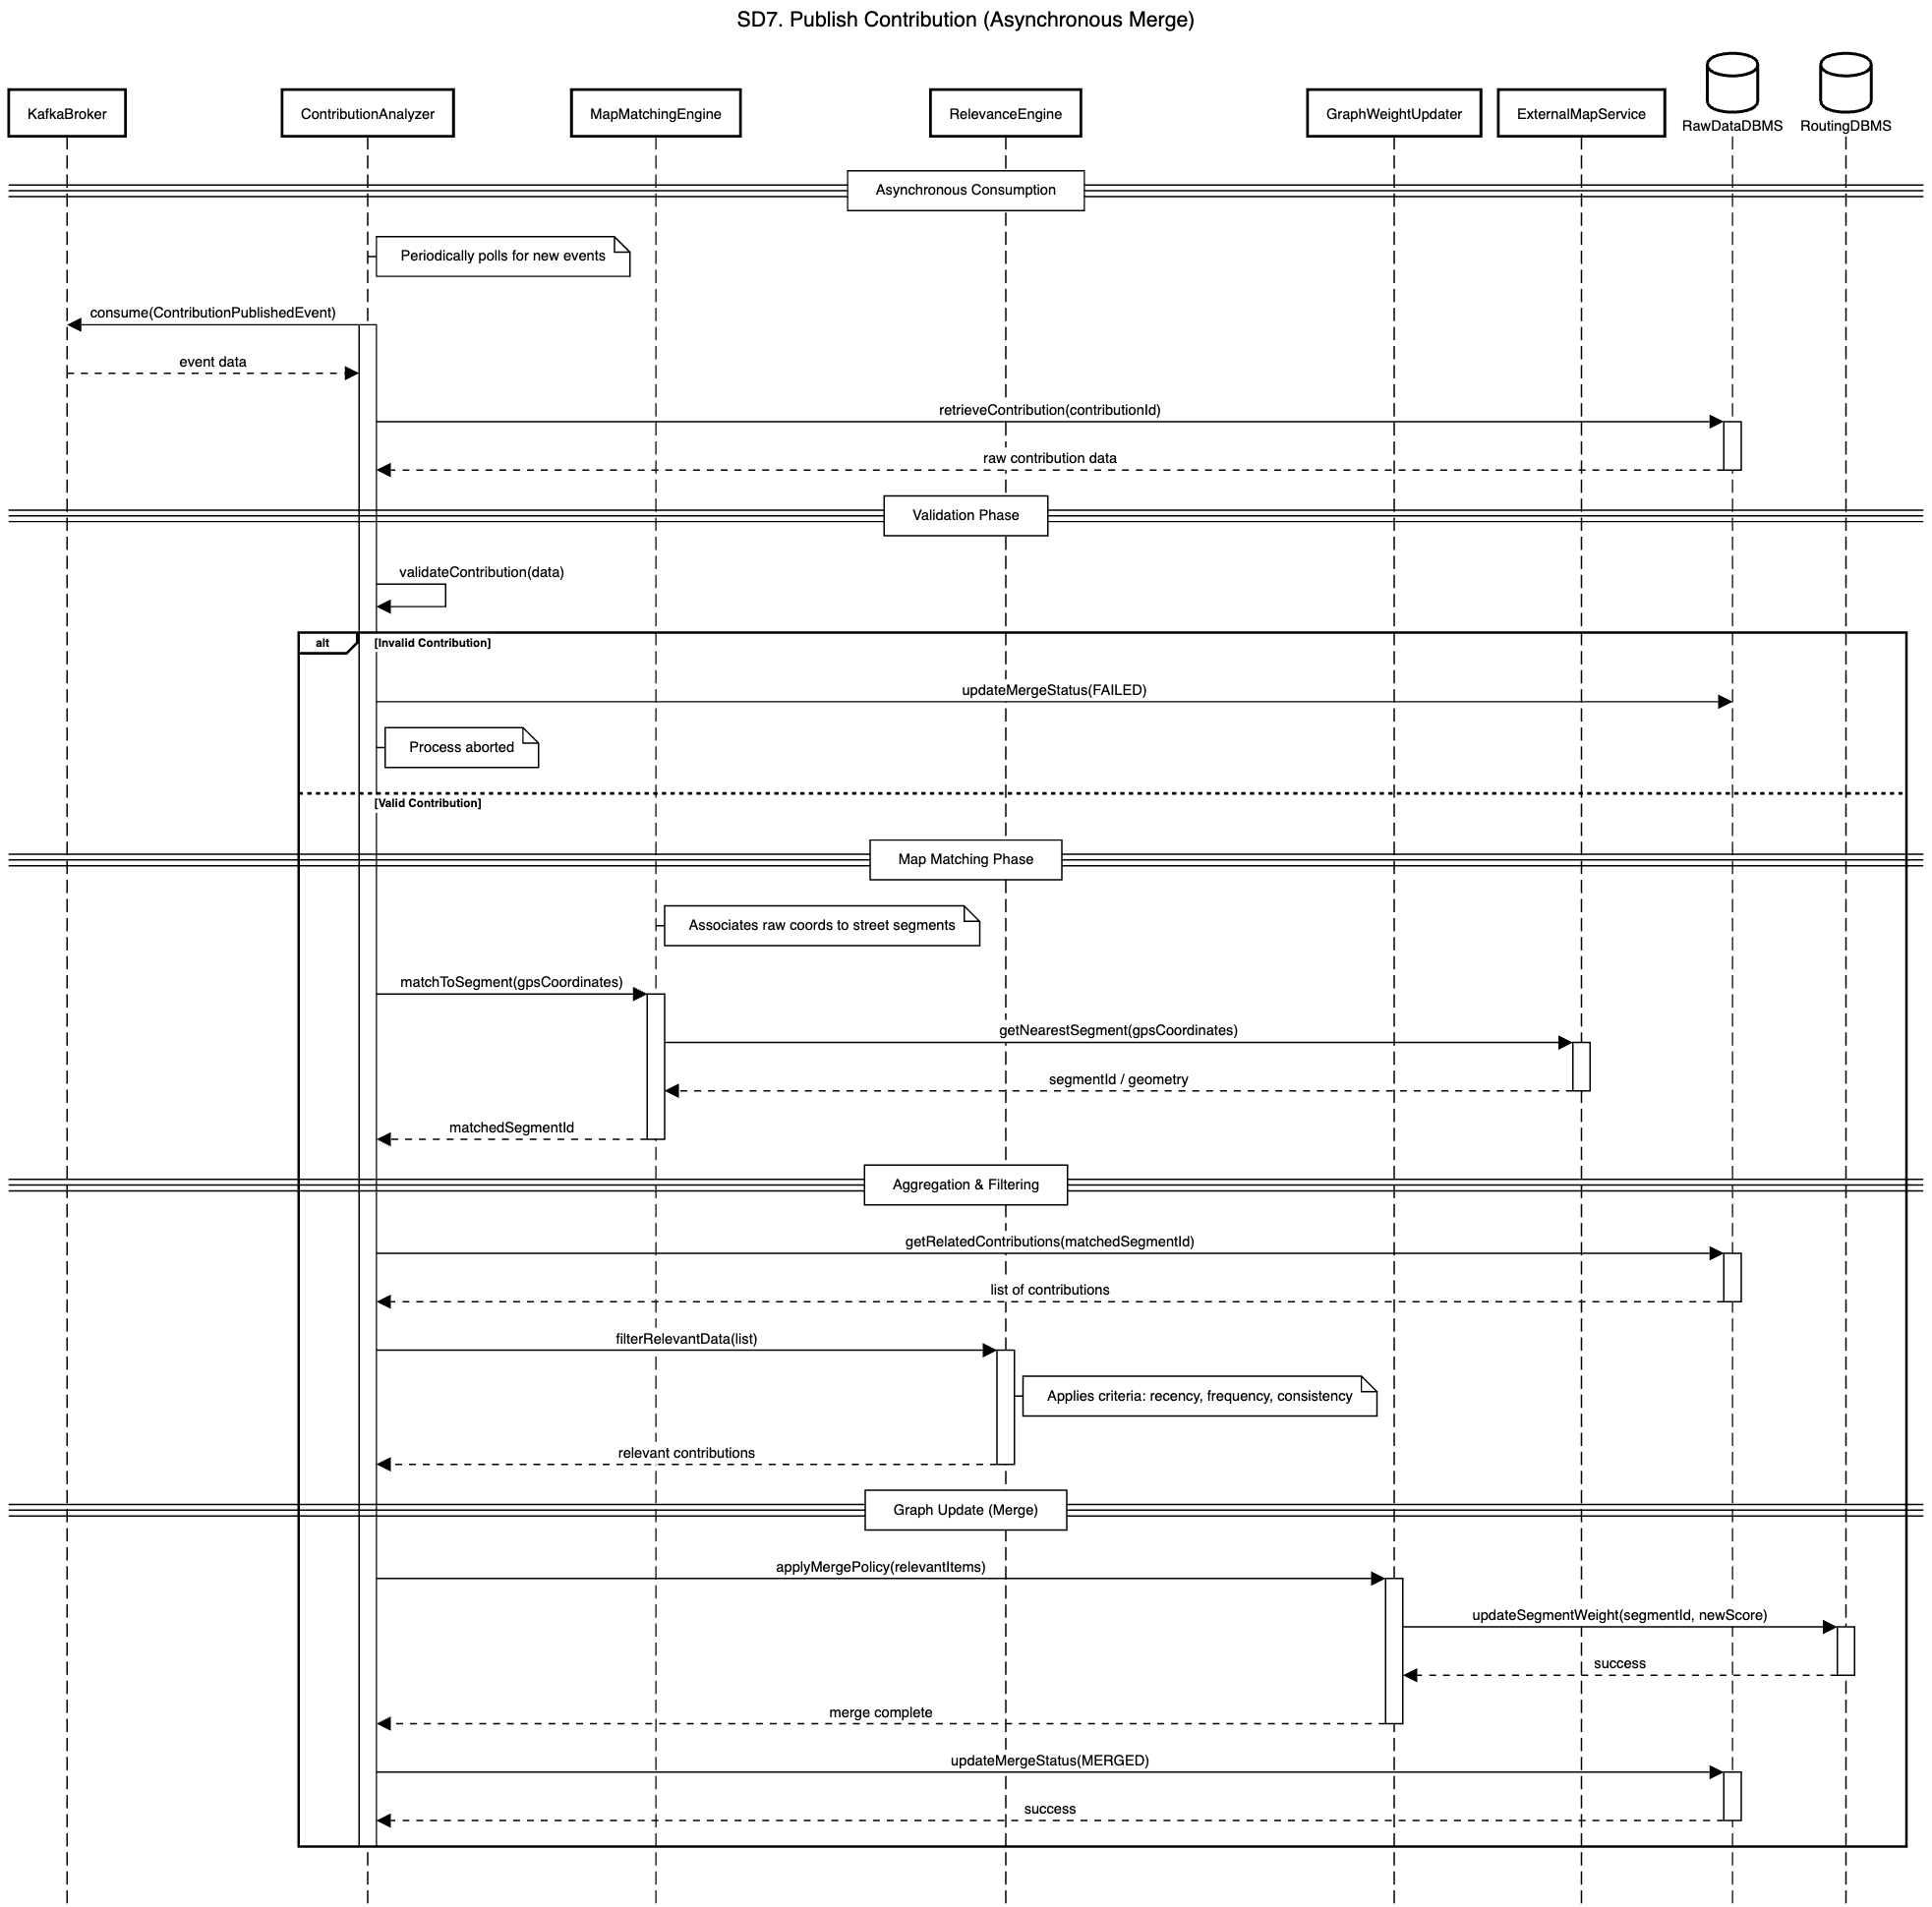
\includegraphics[width=1\linewidth]{DD/Images/sd/sd_publishcontribution.png}
         \caption{Publish Contribution}
         \label{fig:publish_contribution_sd}
     \end{center}
\end{figure}

\newpage

\subsubsection*{SD\cuc. View Map}
\label{subsubsec:view_map_sd}

The Registered User or Unregistered User initiates this interaction by accessing the map section of the Client App or by panning and zooming to a new geographical area. The Client App calculates the bounding box of the currently visible region and issues parallel requests to the backend to retrieve the necessary geospatial data. These requests are forwarded by the API Gateway to the \texttt{MapDiscoveryManager}.

 The \texttt{MapDiscoveryManager} queries the  \texttt{external map service} to obtain the latest map dat of the road network after doing so it uses the \texttt{RoutingDBMS} (the graph-oriented database) to fetch the \texttt{StreetSegment}s located within the specified bounding box to retrieve the overlay information, which includes aggregated contributions such as obstacles, roadworks, and path quality scores, ensuring the map reflects the real-time condition of the road network.

The diagram also illustrates specific user interactions that can occur within the map view. 

If the User taps on a specific path segment, the Client App invokes the \texttt{/map/getSegmentDetails} interface. The \texttt{MapDiscoveryManager} retrieves the detailed attributes and the list of active contributions for that specific segment from the database and returns them to the client for inspection.

If the User initiates a search for a specific route, the system invokes the \texttt{Path Planner} component (refer to the \textit{Search Path} sequence diagram for details). Finally, if the User decides to follow a suggested path, the system redirects the User to the "Automatic Trip Mode" interface, triggering the logic described in the \textit{Follow Path} and \textit{Automatic Insertion} use cases.

\newpage

\begin{figure}[H]
    \begin{center}
         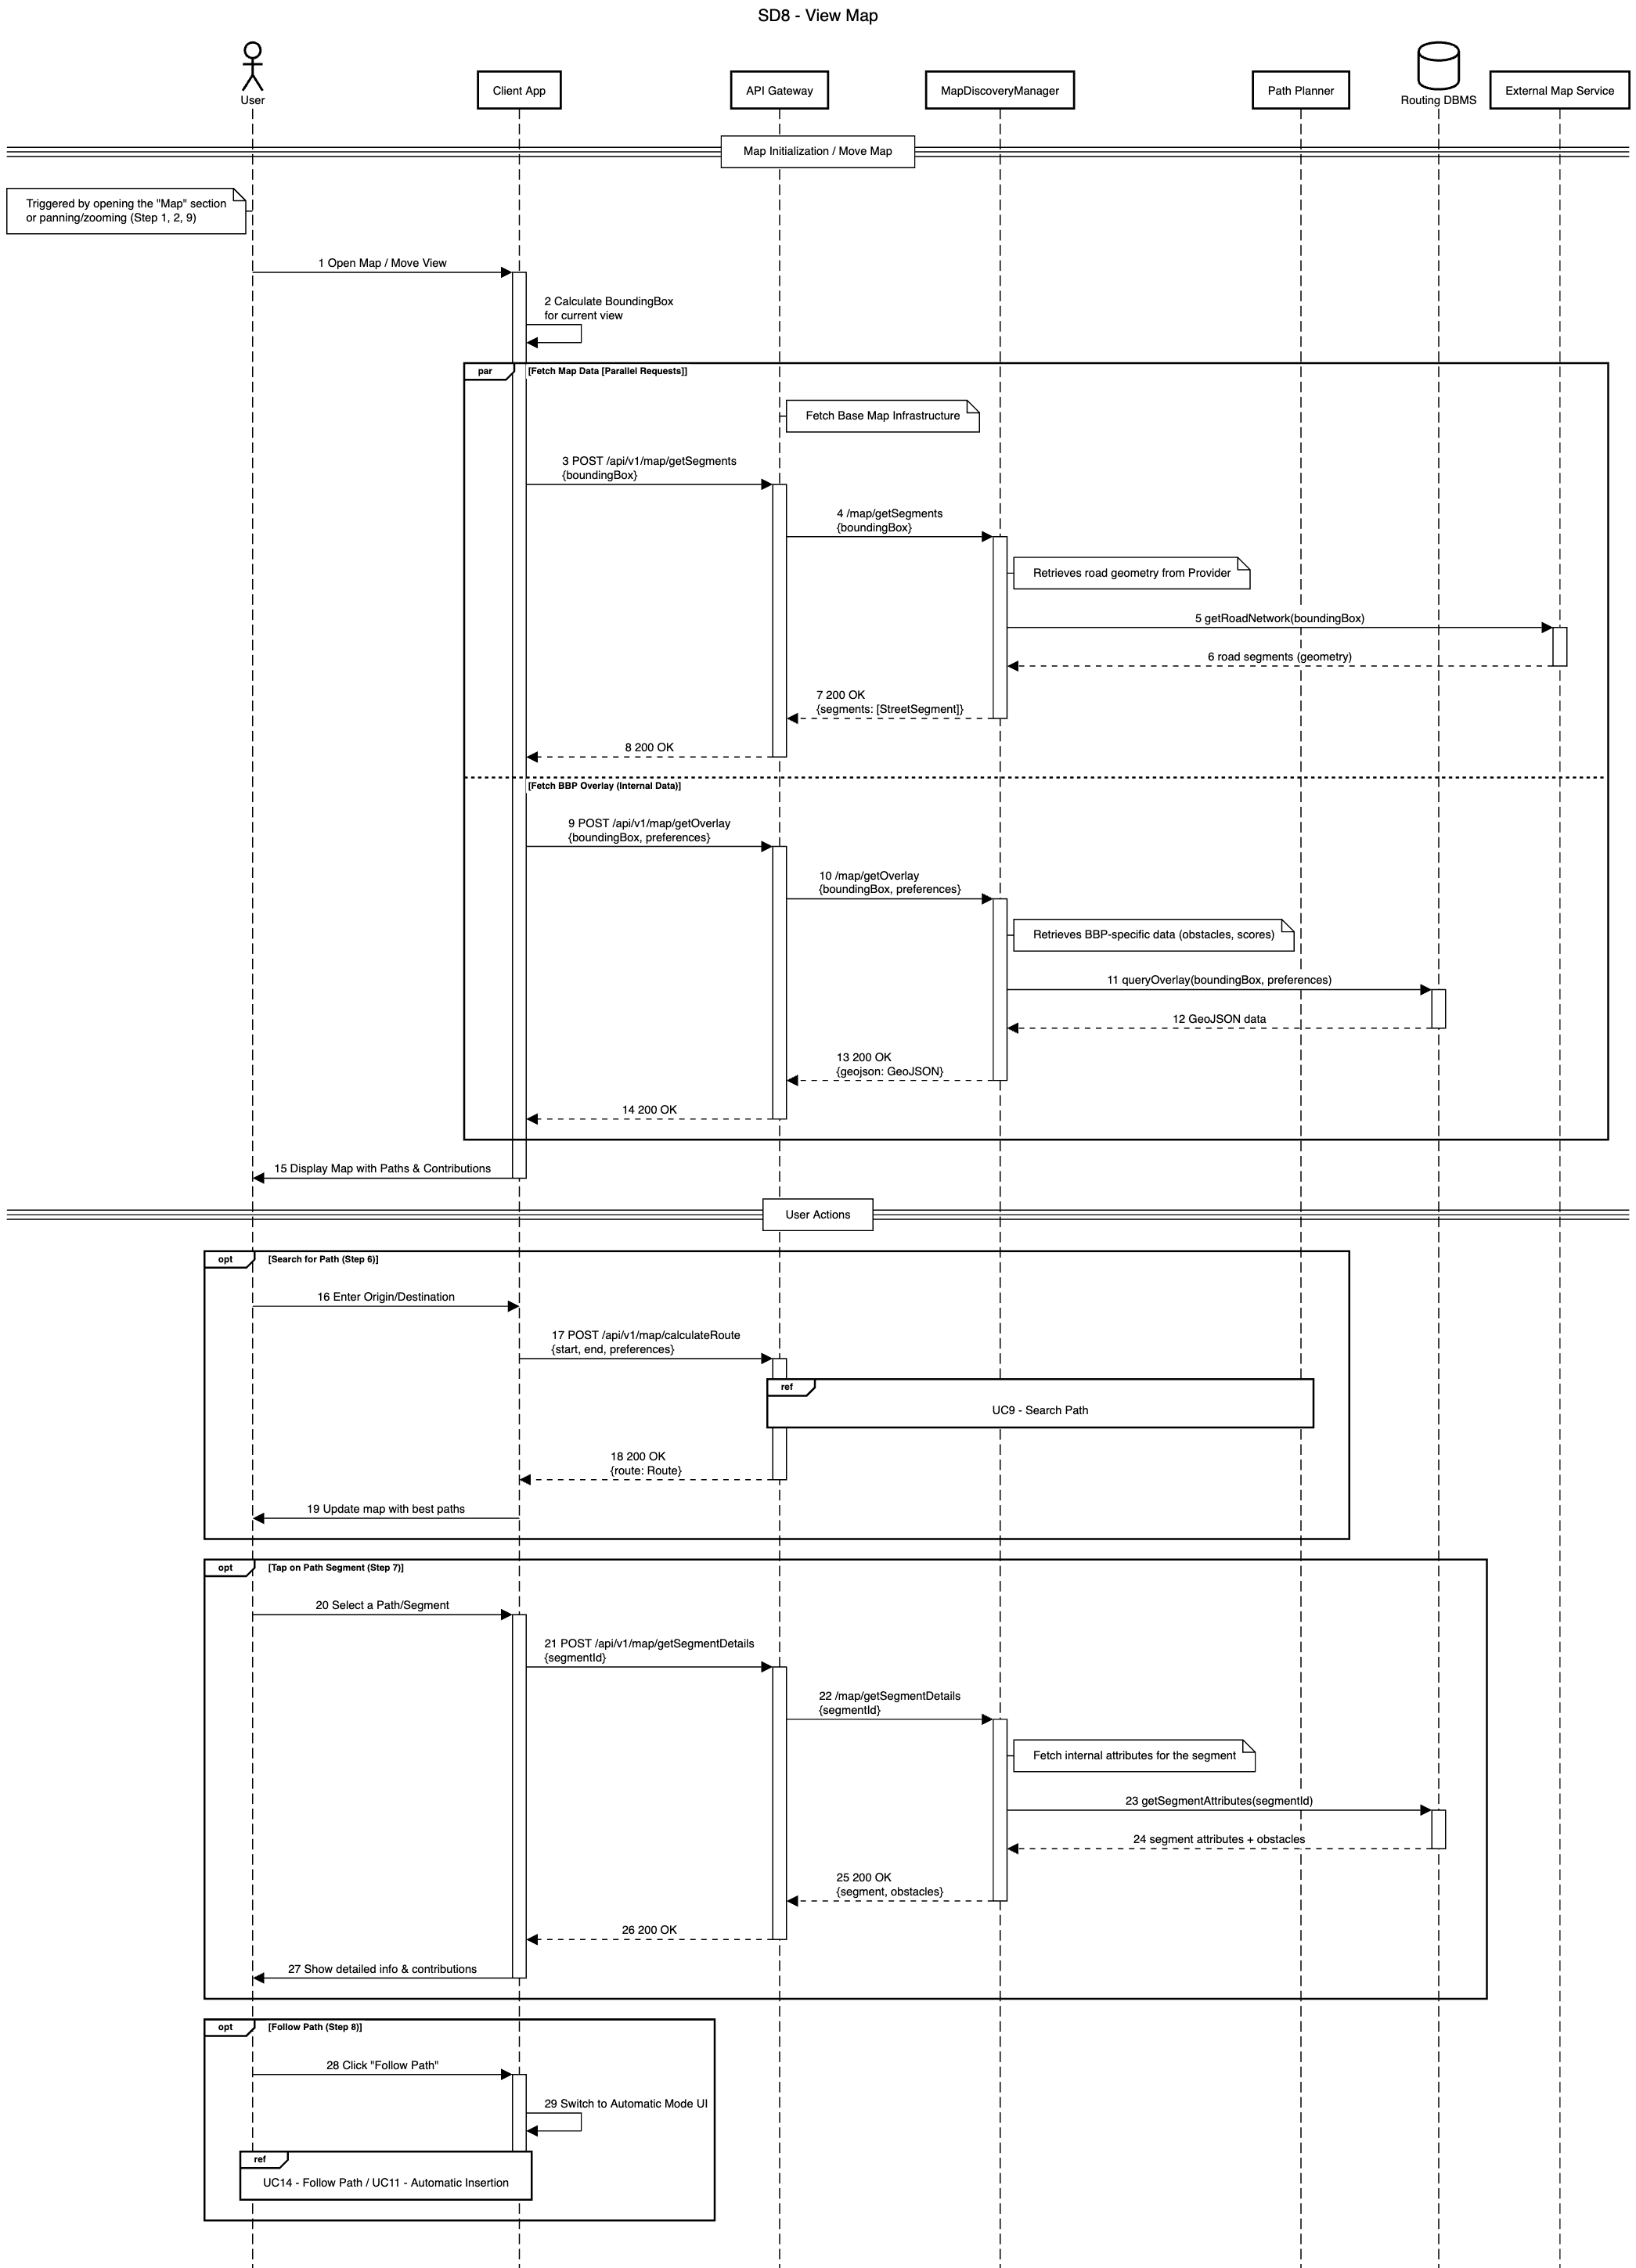
\includegraphics[width=1\linewidth]{DD/Images/sd/sd_viewmap.png}
         
         \caption{View Map}
         \label{fig:view_map_sd}
    \end{center}
\end{figure}

\newpage

\subsubsection*{SD\cuc. Search Path}
\label{subsubsec:search_path_sd}

The interaction begins when the User specifies an origin and a destination within the Client App. The request is sent to the \texttt{PathFinder} service via the API Gateway. The \texttt{Path Planner} first queries the \texttt{RoutingDBMS} to retrieve all geometrically valid paths connecting the two points.

If no bike path exists connecting the specified points, the system returns an empty result, and the Client App displays an informative message to the User to notify them that no route is available.

Conversely, if valid paths are found, the system determines the ranking logic based on the user's registration status. If the user is Unregistered, the paths are ranked using standard criteria (e.g., shortest distance or highest safety score) and returned immediately.

If the user is Registered, the \texttt{PathFinder} orchestrates a personalization process. It invokes the \texttt{ProfileManager} to retrieve the user's specific preferences (e.g., surface type, safety priority) and the \texttt{TripHistoryManager} to fetch data on recently completed trips. Using this contextual data, the \texttt{PathPlanner} reorders the candidate paths to prioritize those that best match the user's habits and settings. Finally, the ordered list of paths is returned to the Client App for display.

\newpage

\begin{figure}[H]
    \begin{center}
         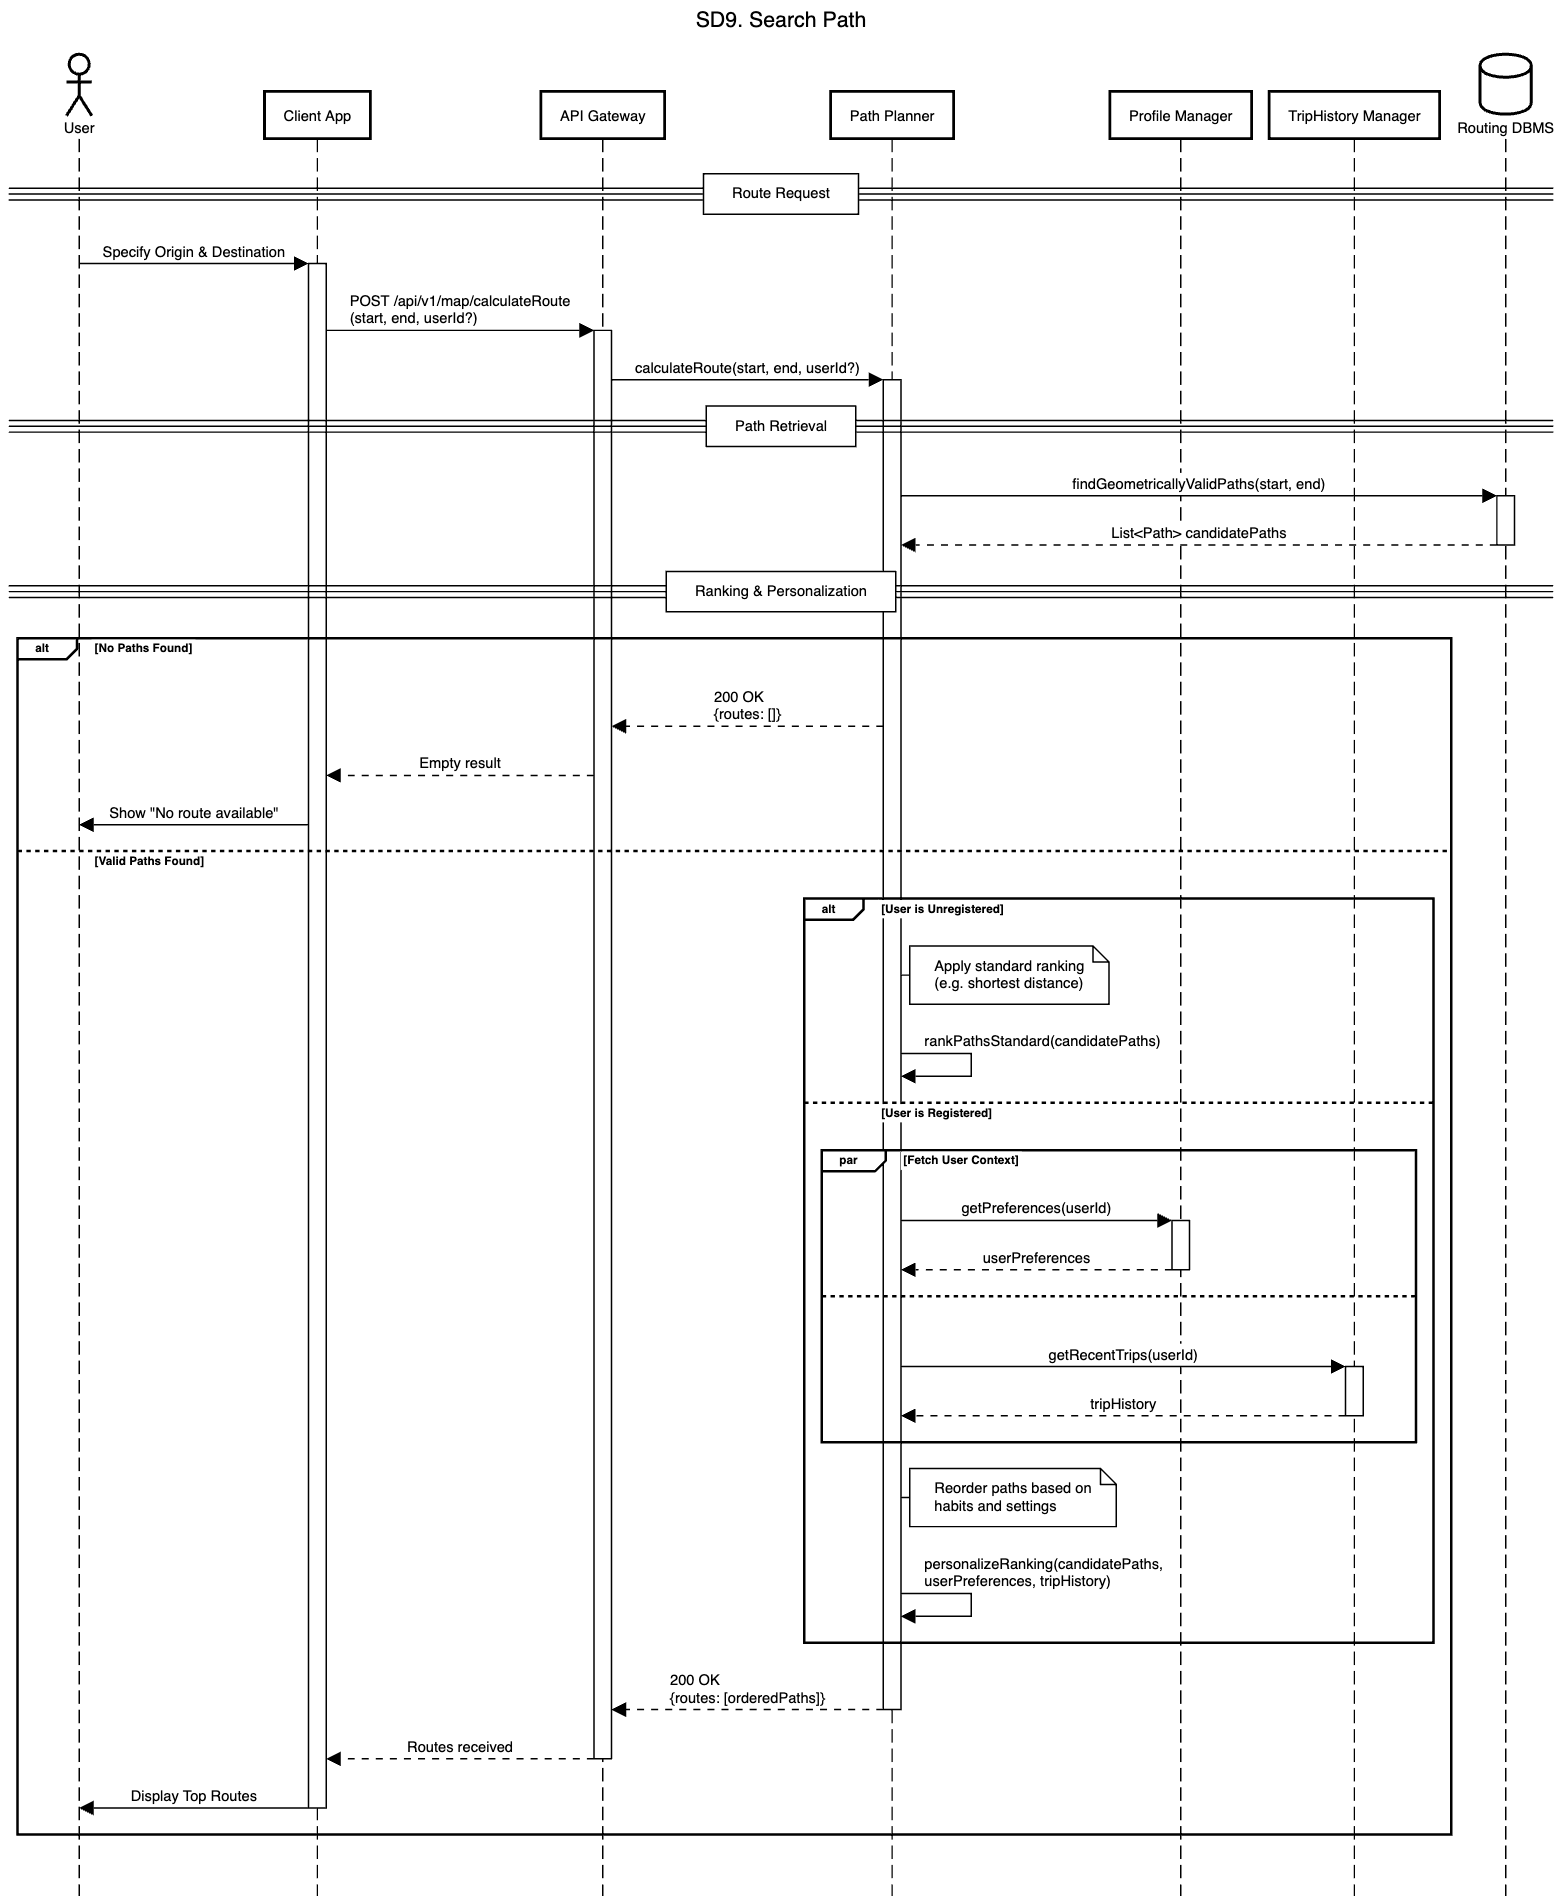
\includegraphics[width=1\linewidth]{DD/Images/sd/sd_searchpath.png}
         \caption{Search Path}
         \label{fig:search_path_sd}
    \end{center}
\end{figure}

\newpage

\subsubsection*{SD\cuc. Manual Insertion}
\label{subsubsec:manual_insertion_sd}

The interaction begins when the Registered User enters the manual insertion mode, triggering the Client App to initialize a local \texttt{TripDraft} state. The user constructs the route iteratively by adding street segments; this allows for two distinct interaction patterns: searching for existing paths (which triggers the logic described in the \textit{Search Path} sequence diagram) or manually selecting segments on the map. In the latter case, the Client App queries the \texttt{MapDiscoveryManager} via the API Gateway to retrieve the necessary segment details.

Once the route definition is confirmed, the Client App locally validates the geometric consistency of the draft. If valid, the user can enrich the trip by adding contributions (e.g., obstacles or roadworks). Each contribution undergoes validation to ensure all mandatory fields are present before being attached to the draft.

The process concludes with the user selecting a final action. If the user chooses to \emph{Save as Trip}, the data is sent to the \texttt{ManualReportManager} with the \texttt{isTrip} flag set to true. The manager persists the trip in the \texttt{RawDataDBMS}. If the user marks the trip as public, the service emits a \texttt{TripPublishedEvent} to the Kafka Broker to trigger asynchronous aggregation.

Alternatively, if the user chooses to \emph{Publish as Report}, the system treats the input as a standalone contribution. The \texttt{ManualReportManager} stores it and immediately publishes a \texttt{ContributionPublishedEvent} to Kafka, allowing the \texttt{Data Aggregation Service} to process it independently of a trip session. Finally, the user may choose to \emph{Discard} the draft, clearing all local data without backend interaction.

Exceptions, such as invalid draft geometries are handled by displaying appropriate error messages to the user, allowing them to correct the data or retry the operation.

\begin{figure}[htbp]
    \centering
    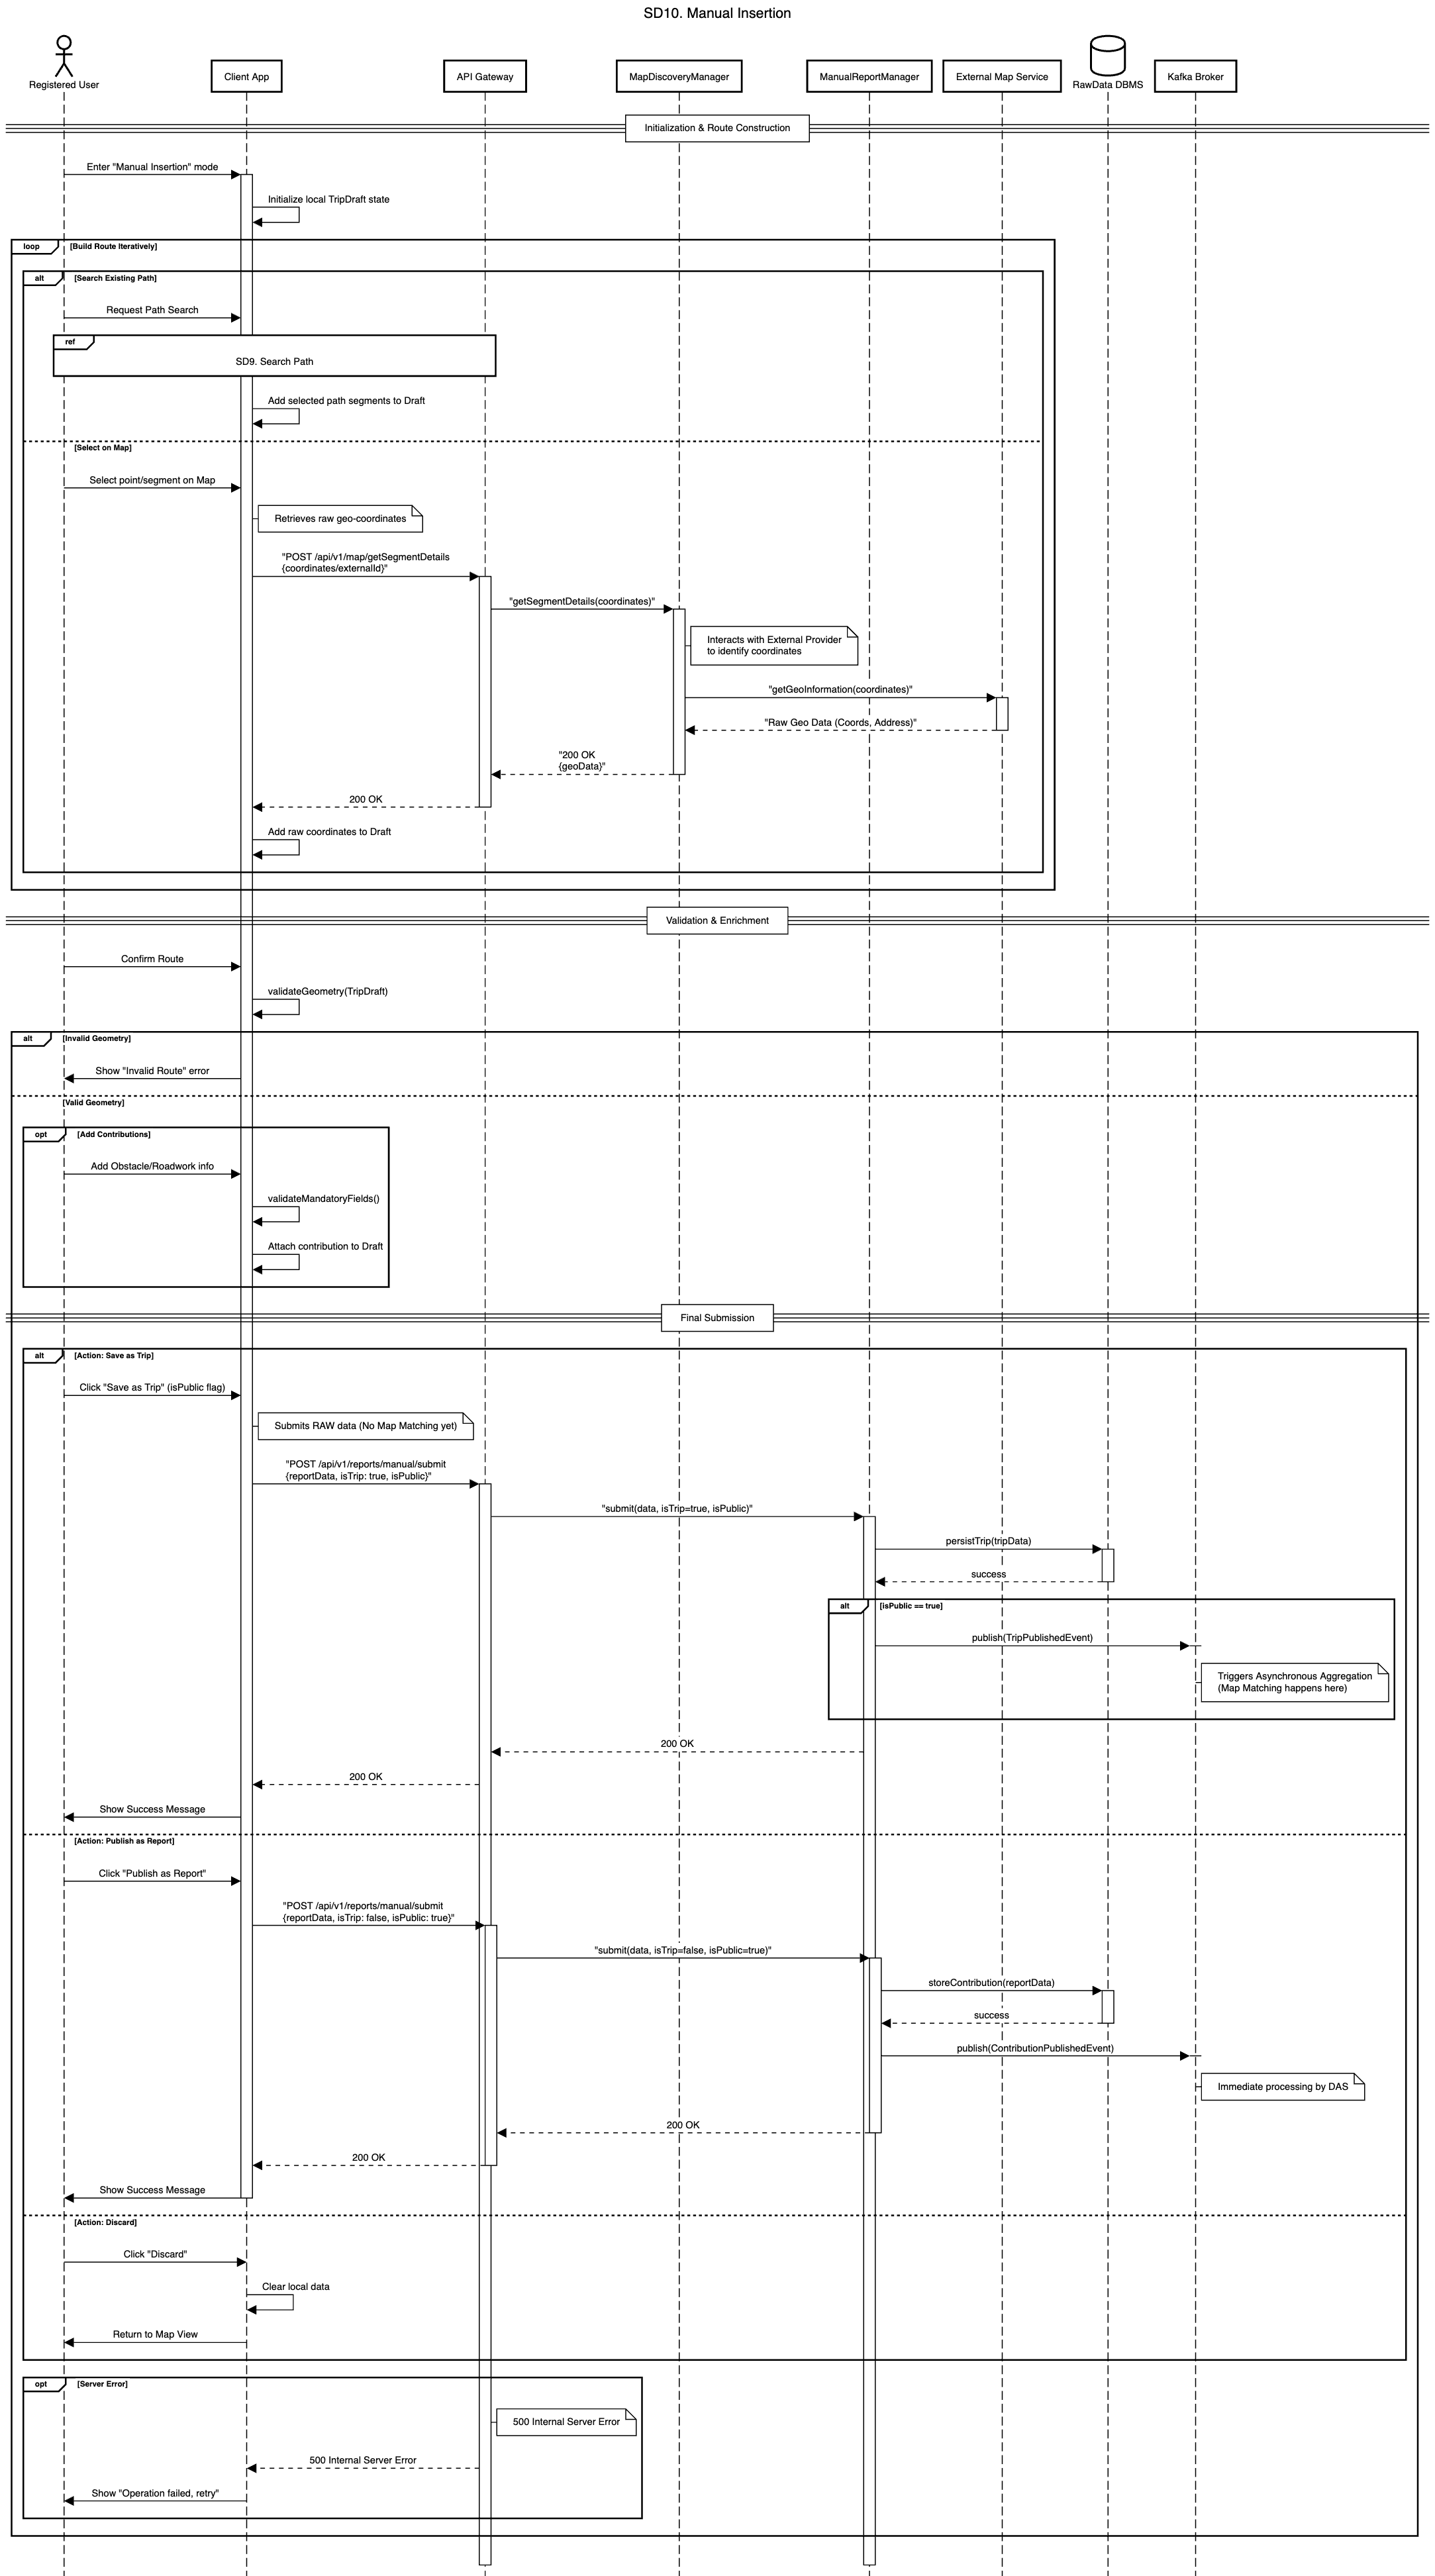
\includegraphics[width=0.8\linewidth]{DD/Images/sd/sd_manualinsertion.png}
    \caption{Manual Insertion}
    \label{fig:manual_insertion_sd}
\end{figure}

\newpage

\subsubsection*{SD\cuc. Automatic Insertion}
\label{subsubsec:automatic_insertion_sd}

The interaction is initiated by the Registered User pressing the "Start recording" button. The Client App performs a preliminary check on hardware availability; if successful, it initializes a local \texttt{RecordingSession} and activates the GPS, accelerometer, and gyroscope sensors.

During the recording phase, the Client App periodically acquires sensor data and buffers it locally. While the Use Case description mentions continuous inference, the architectural design delegates the heavy computational logic to the backend to optimize mobile resources. However, the Client App performs real-time monitoring of the user's movement to detect interruptions (stationary status) based on GPS position changes over a configurable time window.

When the user stops the recording, the Client App halts the sensors and submits the collected raw data to the \texttt{AutomaticTripProcessor} via the API Gateway. The backend processor reconstructs the full path and calculates trip statistics (e.g., distance, average speed).

Subsequently, the \texttt{AutomaticTripProcessor} invokes the \texttt{Inference Engine} to analyze the raw sensor logs and detect potential obstacles (e.g., potholes, bumps), generating a set of draft Contributions. It also orchestrates the data enrichment process by triggering the logic described in the \textit{Enrich Trip with Weather Information} sequence diagram.

Finally, the processed trip and the inferred contributions are stored as a draft in the \texttt{RawDataDBMS}, and the result is returned to the Client App. The system then redirects the user to the "Review and Edit" screen (refer to \textit{UC13 - Edit Trip}), allowing them to validate or modify the automatically generated data.

Exceptions related to sensor unavailability are handled locally by the Client App, preventing the recording from starting.

\newpage

\begin{figure}[H]
    \begin{center}
         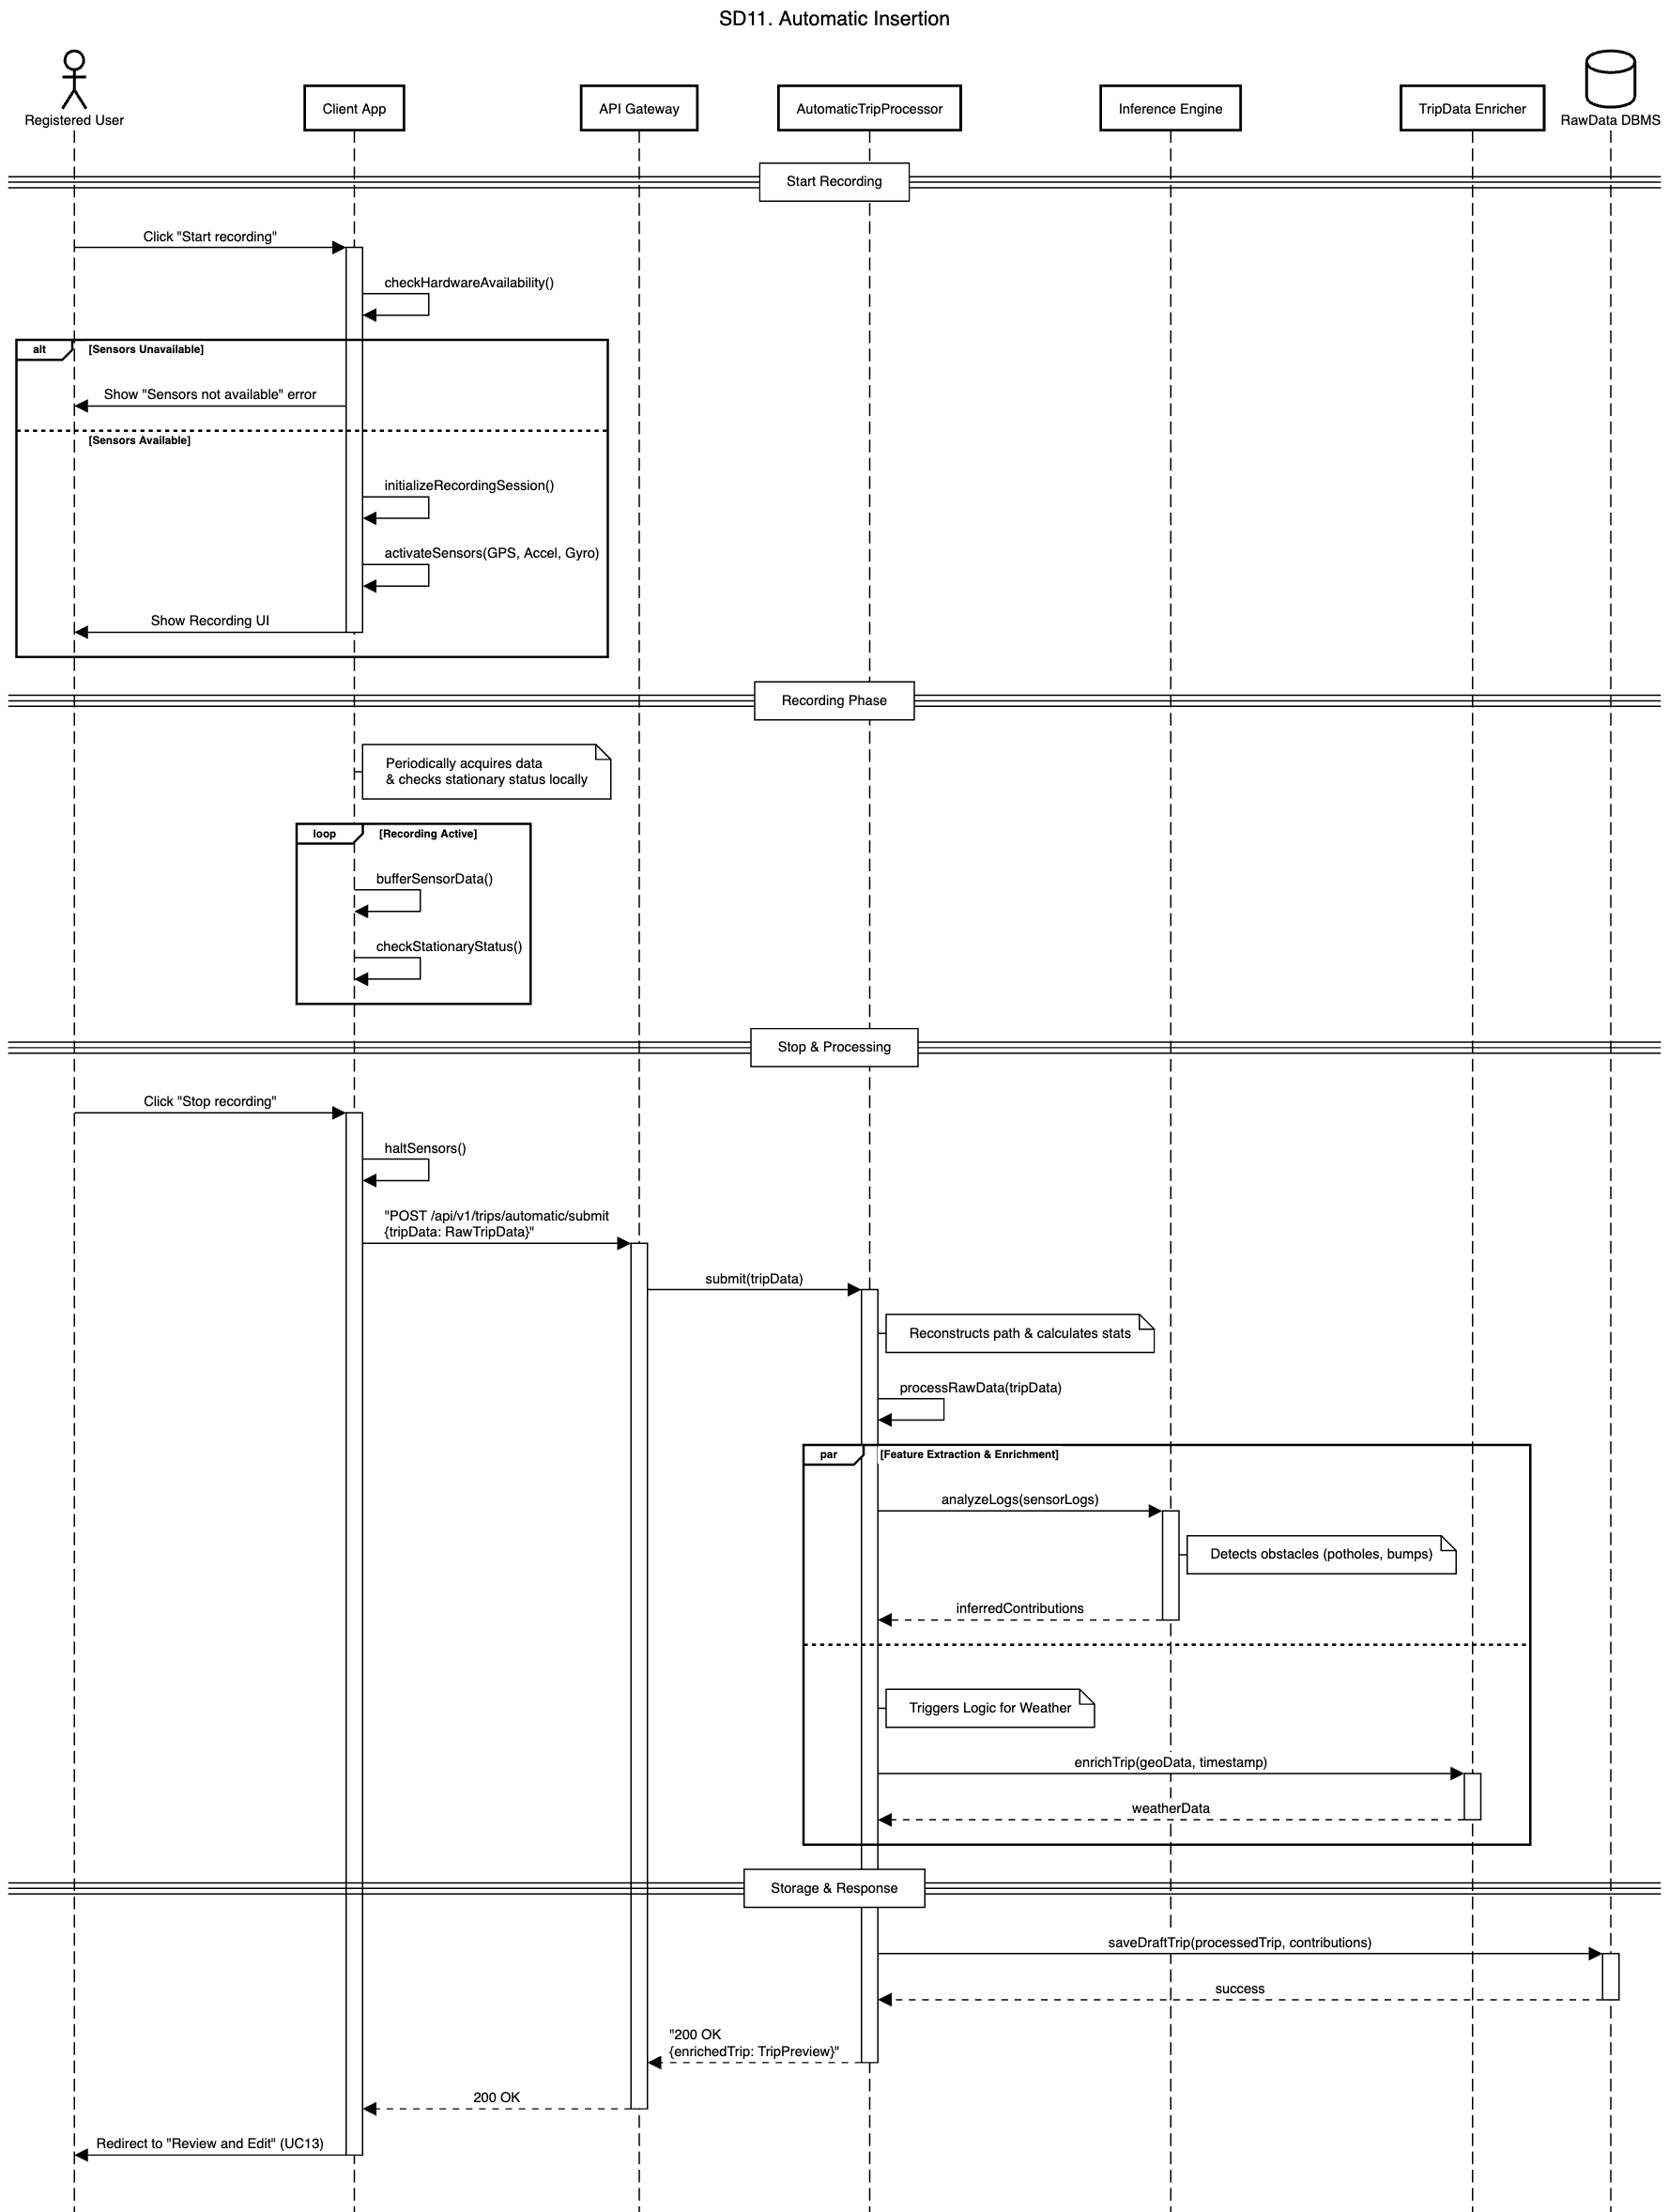
\includegraphics[width=1\linewidth]{DD/Images/sd/sd_automaticinsertion.png}
         \caption{Automatic Insertion}
         \label{fig:automatic_insertion_sd}
    \end{center}
\end{figure}

\newpage

\subsubsection*{SD\cuc. Enrich Trip with Weather Information}
\label{subsubsec:enrich_weather_sd}

This process is typically invoked by the \texttt{AutomaticTripProcessor} immediately after reconstructing the path of a completed trip. The \texttt{Data Enrichment Service} receives the trip draft containing the GPS trace and the corresponding timestamps.

First, the service validates the input data to ensure the GPS trace contains sufficient information to locate the trip geographically and temporally. If the data is valid, the service constructs a request and queries the external \texttt{Weather Service} API to retrieve historical weather conditions (e.g., temperature, wind speed, precipitation) matching the trip's time and location.

If the external service responds successfully, the retrieved meteorological data is parsed and attached to the trip object, enriching the final summary presented to the user.

However, if the external service is unavailable, returns an error, or if the initial GPS data is incomplete, the system adopts a graceful degradation strategy. The trip is marked as "No Weather Data Available," and the process completes without the enrichment, ensuring that the core trip data is preserved and can still be saved successfully.

\newpage

\begin{figure}[H]
    \begin{center}
         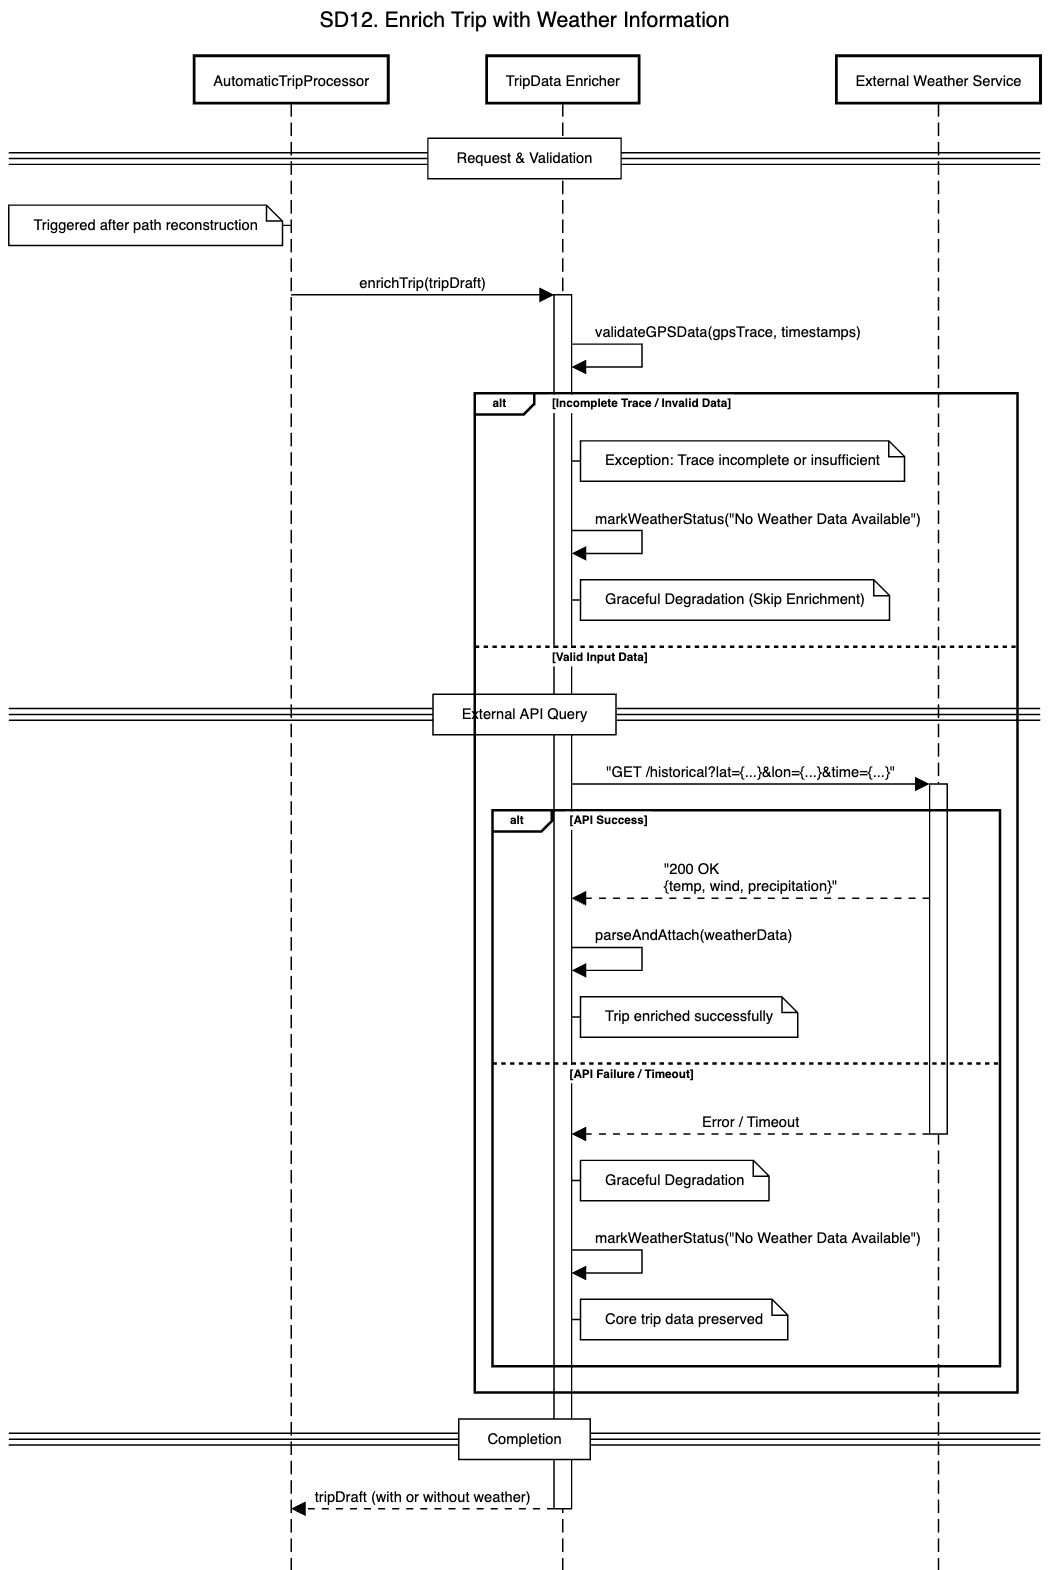
\includegraphics[width=0.8\linewidth]{DD/Images/sd/sd_weatherinfo.png}
         \caption{Enrich Trip with Weather Information}
         \label{fig:enrich_weather_sd}
    \end{center}
\end{figure}

\newpage

\subsubsection*{SD\cuc. Edit Trip}
\label{subsubsec:edit_trip_sd}

This interaction begins immediately after an automatic trip recording concludes. The Client App presents the user with a review screen displaying the reconstructed path and the set of automatically detected obstacles (e.g., potholes, bumps).

The user can interactively modify the draft data locally: detected obstacles can be confirmed, adjusted, or removed if incorrect. Additionally, the user can manually add missing contributions that the automatic inference might have missed. These changes are maintained in the local application state until a final decision is made.

Once the review is complete, the user selects a final action. If \textbf{Store and Publish} is chosen, the finalized data is sent to the \texttt{AutomaticTripProcessor}. The processor updates the trip record in the \texttt{RawDataDBMS} and marks it as public. Crucially, it then iterates through the valid contributions and the trip itself, emitting corresponding events to the Kafka Broker to trigger the asynchronous aggregation process.

If the user selects \textbf{Store Only}, the updated trip data is persisted in the database but marked as private, skipping the publication to Kafka. If \textbf{Discard} is chosen, the backend is instructed to permanently delete the draft trip and all associated data from the database.

Exceptions, such as database write failures, are handled by returning an error response to the client, prompting the user to retry the operation to prevent data loss.

\newpage

\begin{figure}[H]
    \begin{center}
         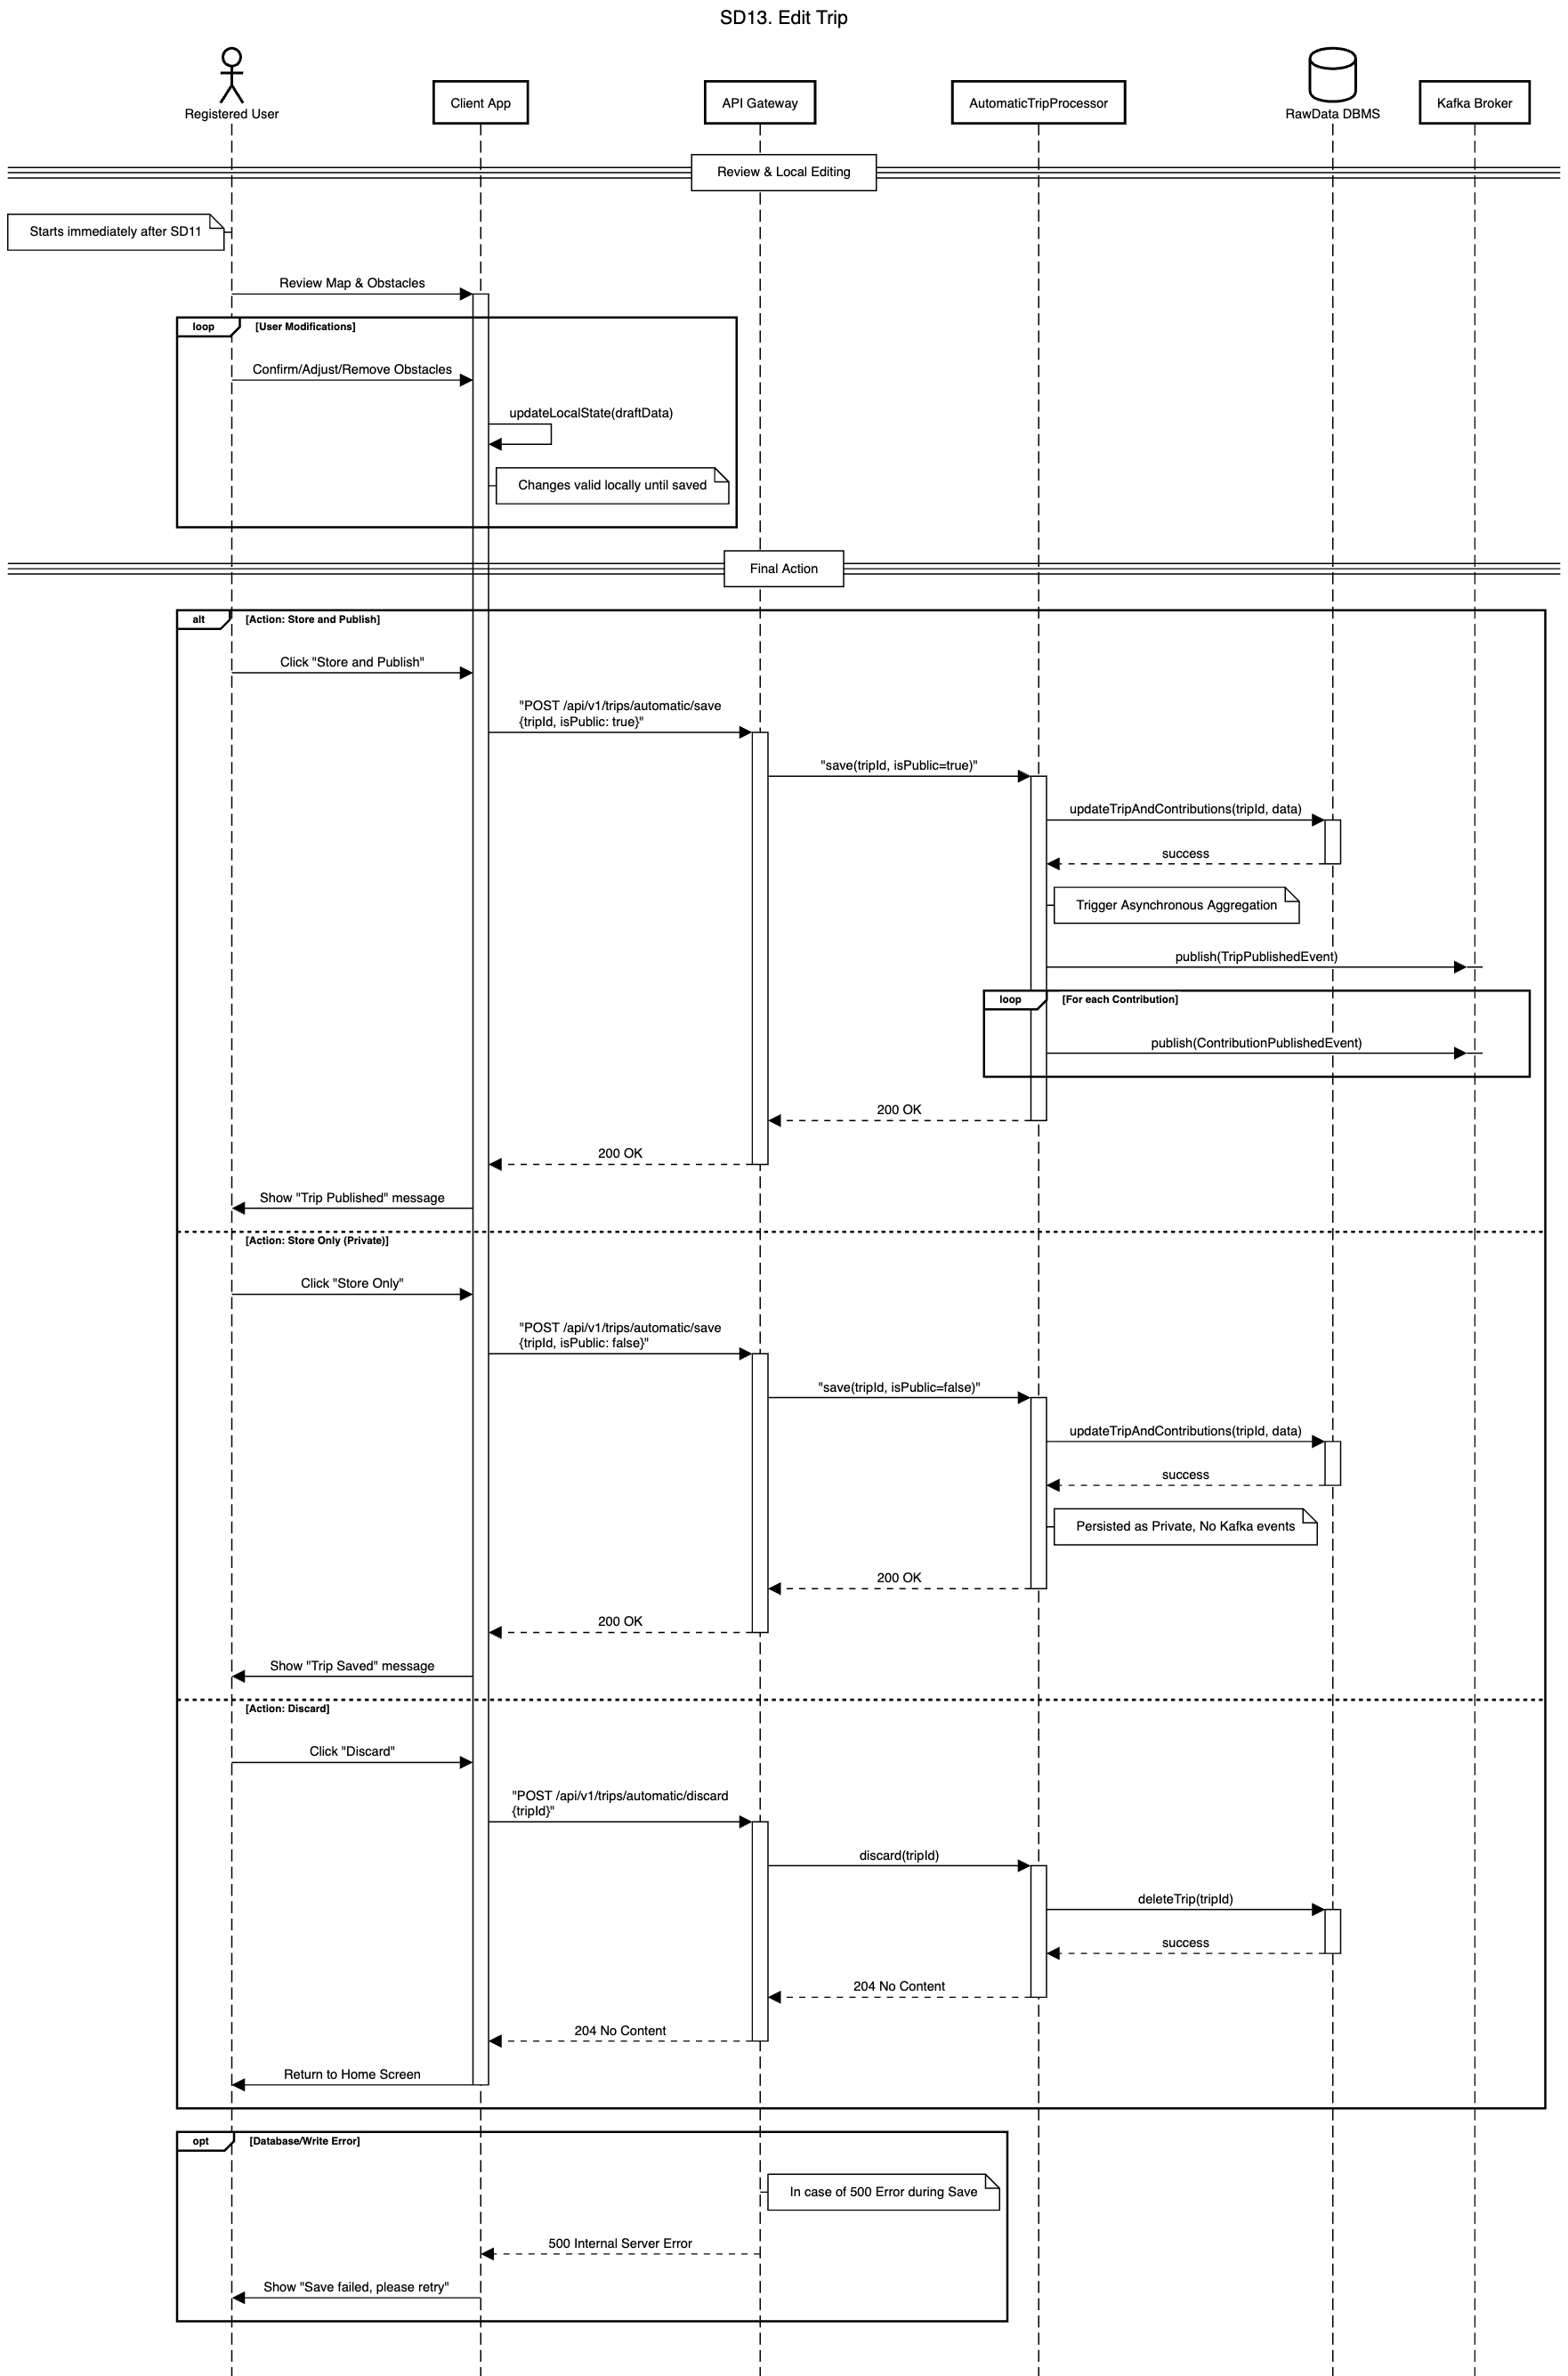
\includegraphics[width=0.8\linewidth]{DD/Images/sd/sd_edittrip.png}
         \caption{Edit Trip}
         \label{fig:edit_trip_sd}
    \end{center}
\end{figure}

\newpage
\section{Selected Architectural Styles and Patterns}

For BBP, various styles and patterns allow for better management of the key aspects of the system:

\begin{itemize}
    \item \textbf{Polyglot Persistence}:  
    BBP uses  different data storage technologies depending on the specific needs of each subsystem, utilizing relational databases to handle profile and security data, graph DBs to store route data and document databases for the rest. This choice enables the system to optimize performance, scalability, and data modeling by selecting the most appropriate database technology for each domain. As a result, schema evolution and performance tuning can be handled independently, reducing the impact of changes and improving overall system flexibility.

    \item \textbf{Eventual Consistency}:  
    BBP is designed as a distributed system, where strong consistency across all components would negatively impact availability and fault tolerance. According to the CAP theorem, it is impossible to guarantee consistency, availability, and partition tolerance simultaneously. BBP prioritizes availability and partition tolerance, adopting an eventual consistency model temporary inconsistencies in data such as not immediately updated routes are acceptable and do not compromise the correctness of the system’s behavior.

    \item \textbf{Local Caching for Map Matching}:
    To reduce latency and limit the dependency on external map services, the component responsible for map matching (\textit{Map Matching Engine}) adopts a local caching strategy.

    The cache stores associations between spatial coordinate ranges and the corresponding street segments previously resolved. When new GPS data falls within a cached range, the system can reuse the stored mapping instead of issuing a new external API request.
    This approach significantly improves performance for frequent and geographically localized requests, while also increasing system robustness in the presence of temporary unavailability or rate limiting of external map providers.


    \item \textbf{API Gateway Pattern}:  
    The API Gateway pattern is adopted as a single entry point for all client requests.
    Its implementation can rely on widely adopted reverse proxy and gateway solutions, without constraining the architecture to a specific technology.
    For instance, such a gateway could be implemented using a reverse proxy solution (e.g., NGINX), although alternative technologies are equally suitable.

    \item \textbf{Circuit Breaker Pattern}:  
    The Circuit Breaker pattern is applied at the API Gateway level to protect the system from cascading failures caused by unavailable or slow downstream services, including external providers.
    Although BBP does not offer safety-critical functionalities, this mechanism improves system robustness and availability by isolating failures and enabling graceful degradation, for instance by temporarily disabling non-essential features such as weather enrichment.

    
    \item \textbf{Asynchronous Processing via Message Broker}:  
    To decouple time-sensitive operations from computationally expensive background tasks, BBP adopts an asynchronous messaging approach.
    In particular, the persistence of recorded trips is handled synchronously to ensure a responsive user experience, while the subsequent merging and aggregation of path information is triggered asynchronously through events published to a message broker.
    This design follows an event-driven architecture, improving scalability and fault isolation by allowing the merging process to evolve independently from trip ingestion. Temporary delays in the merging phase do not compromise system correctness, as path aggregation naturally tolerates eventual consistency.

    
\end{itemize}
